\chapter{Simulations of Cross-Beam Energy Transfer for Magnetised Direct-Drive}

This chapter describes a set of simulations which were conducted to understand the role of \ac{CBET} in magnetised, direct-drive implosions.
Magnetised \ac{ICF} is a promising route to achieving higher target gains, due to the reduction of thermal energy loss at stagnation and additional confinement of the alpha particles responsible for burn propagation.
For direct-drive implosions, magnetisation can significantly alter the coronal plasma conditions, due to the introduced anisotropy of thermal transport.
The \ac{IAW} dispersion relation, which mediates \ac{CBET} interactions, depends upon the background plasma and therefore significantly altered temperature and density profiles could alter the action of \ac{CBET}.
Before the development of \textsc{Solas}, no direct-drive suitable \ac{CBET} model existed, which was integrated into a \ac{Rad-MHD} code.
Therefore, the \textsc{Chimera}-\textsc{Solas} framework has enabled the effect of magnetisation on \ac{CBET} to be studied for a direct-drive implosion.

The chapter begins with a review of experimental and computational work on magnetised \ac{ICF}, with a particular focus on magnetised direct-drive.
Work presented in this chapter focuses on the study of \textit{exploding-pusher} experiments.
These are very different implosions to the typical \textit{central hot-spot} ignition designs, presented in previous chapters, so a short summary of exploding pushers is also provided.
Simulation results are presented of 1-D and 2-D, unmagnetised exploding pushers, both with and without the effect of \ac{CBET}, which demonstrate that \ac{CBET} does significantly alter these implosions.
This is followed by an investigation of how various extended-\ac{MHD} terms affect the implosion, including the Nernst effect, the Lorentz force and resistive diffusion of the magnetic field.
Results are given of how magnetisation affects the \ac{CBET} interaction and ultimately how it changes the stagnation shape of the target.
The results presented, demonstrate that redistribution of deposited power due to \ac{CBET} reduced the amplitude of the stagnation asymmetry, which originated from the polar beam configuration used.
However, the reduction of asymmetry was consistent for different initial seed magnetic field values, and therefore \ac{CBET} was not observed to be sufficiently strongly affected by magnetisation, to lead to observable signatures in experimental measurements.
The chapter concludes with a summary of the work and suggestions of additional experimental configurations, which may leave a more significant signature of magnetisation altering \ac{CBET}.

\newpage

%###############################################################################################################################
%###############################################################################################################################
%###############################################################################################################################
\section{Magnetised Inertial Confinement Fusion and Exploding Pushers}%
\label{sec:Res2_MagICF}

This chapter begins with a review of published studies of relevance to the work conducted in this chapter.
Firstly, a short review of magnetised-\ac{ICF} is presented, which reviews both the key concepts, existing studies and potential challenges of the design.
Both work on direct- and indirect drive is summarised, alongside recent theoretical progress on understanding how magnetisation can effect \ac{LPIs}.
The exploding pusher concept is then briefly explored to aid understanding of the implosion physics, which is markedly different to conventional hot-spot \ac{ICF}.

%################################################################################
%################################################################################
\subsection{Potential Benefits of Target Magnetisation}%
\label{sec:Res2_magbenefits}

\begin{figure}[t!]
    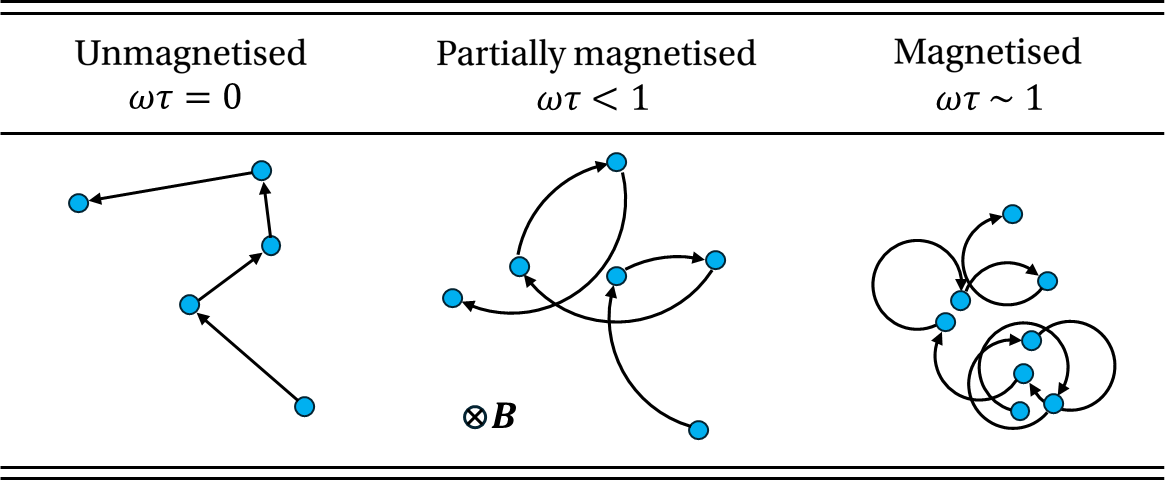
\includegraphics[width=0.75\linewidth]{Results2/Images/wt_collisions.png}
    \centering
    \caption{Cartoon to illustrate the effect of magnetisation on collisions, and therefore transport, of a test positive charge.
    Particle locations after collision are represented as blue circles and the path taken by the particle is shown by the black arrows.
    As the Hall parameter of the particle increases, diffusion is increasingly limited, and therefore collision transport is reduced.}%
    \label{fig:Res2_omegatau}
\end{figure}

Magnetisation of an \ac{ICF} target has long been thought of as a potential aid to ignition~\cite{lindemuth_parameter_1983,jones_physics_1986}.
It is still a relevant field of study in the context of regular ignition events on the \ac{NIF}, because by relaxing the ignition threshold, magnetisation could make larger targets feasible at equivalent laser energy, and therefore lead to higher gains than unmagnetised implosions.
For a central hotspot ignition targets, ignition occurs when the heat source of alpha energy deposition balances the thermal and radiative losses in the hotspot.
Thermal conduction is suppressed perpendicular to magnetic field lines, therefore a magnetic field can reduce thermal losses and aid the power balance required for ignition.
Fig.~\ref{fig:Res2_omegatau} demonstrates the effect of increasing magnetisation on a unit positive test charge.
By constraining charged particles to orbit field lines, collisional transport terms, such as thermal conduction, are reduced perpendicular to the field direction.
Fits of transport coefficients to Fokker-Planck simulations, demonstrate that in a Hydrogen plasma, thermal conductivity perpendicular to field lines $\kappa_{\perp}$, is reduced to $\sim$30\% of the parallel value $\kappa_{\parallel}$ at Hall parameter $\omega\tau=1$, and $\sim$1\% at $\omega\tau=10$~\cite{epperlein_plasma_1986}.
Thus, for Hall parameters, $\omega\tau\gtrsim 10$, thermal conduction losses are almost negligible in the direction perpendicular to field lines.

Using an order of magnitude estimate for a below ignition threshold hotspot, $T_e\sim 2.5\ \text{keV}$ and $\rho\sim50\ \text{g cm}^{-3}$, a field strength $|\vec{B}|\sim 2.5\ \text{kT}$ is required to obtain $\omega\tau\sim1$~\cite{oneill_modelling_2023}.
This field strength cannot be produced directly, but it is possible to produce a smaller field which, assuming frozen in magnetic field and a spherical compression, is amplified by the square of the convergence,
\begin{equation}
    \label{eq:Res2_flux_compression}
    |\vec{B_1}|=|\vec{B_0}| \left(\frac{R_0}{R_1}\right)^2,
\end{equation}
where $|\vec{B_0}|$ and $|\vec{B_1}|$ are initial and final magnetic fields respectively and $R_0$ and $R_1$ are initial and final radii respectively.
Laboratory magnetic fields can be produced from pulsed power coils with field strength $|\vec{B}|\sim\mathcal{O}(50)\ \text{T}$~\cite{fiksel_note_2015}, so even moderate convergence-ratio targets ($R_0/R_1\sim10$) are able to produce strongly magnetised core plasma.

\begin{figure}[t!]
    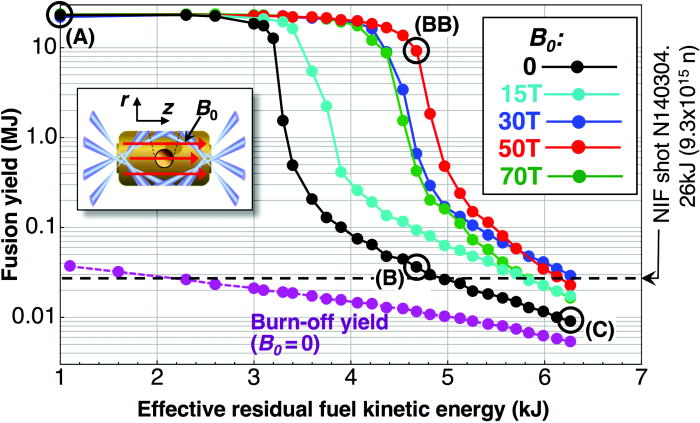
\includegraphics[width=0.75\linewidth]{Results2/Images/magicf_perkins.jpeg}
    \centering
    \caption{Simulated fusion yields versus effective residual fuel kinetic energy under imposed low-mode radiation flux perturbations for imposed fields in the range $B_0=0\rightarrow70\ \text{(T)}$.
    The plot demonstrates with increasing departure from ideal compression (moving to the right on the $x$ axis), magnetisation can enable the onset of the ignition.
    Reused with permission from Ref.~\cite{perkins_potential_2017}.}%
    \label{fig:Res2_perkins_magicf}
\end{figure}

Fig.~\ref{Res2:perkins_magicf} plots results of magnetised indirect-drive simulations, of a target on the threshold of ignition~\cite{perkins_potential_2017}.
Increasing magnitude of radiation perturbation were applied to the drive (moving to the right on the $x$-axis), which prevent the target from achieving ignition, which is visible as the steep increase in yield, below some threshold level of perturbation.
The results demonstrate that when an initial magnetic field was applied to the target, it more robustly ignited with increasing field strength due to reduced conduction losses.
This simulation work, prior to the achievement of ignition on the \ac{NIF}~\cite{zylstra_burning_2022}, motivated the development of a magnetised \ac{ICF} campaign at \ac{LLNL}~\cite{moody_magnetized_2022}.

The \textsc{Chimera} code has been used to study a wide array of physics relevent to magnetised \ac{ICF}.
Simulation work has been conducted, which has shown that magnetisation can alter instability growth of magnetised laser fusion implosions.
While in the deceleration phase, magnetic tension can reduce low-mode perturbation growth~\cite{walsh_perturbation_2019}, magnetisation of directly-driven targets inhibits heatflow in the plasma corona and thus limits thermal stabilisation of short wavelength modes from laser imprint~\cite{walsh_magnetized_2020}.
Recent work has also demonstrated that magnetisation of high-yield, indirect-drive targets must be carefully optimised, in order to avoid significant degradation to the implosion shape, due to anisotropic thermal conduction and inhibition of burn propagation, due to $\alpha$ magnetisation~\cite{oneill_modelling_2023}.

%################################################################################
%################################################################################
\subsection{Experimental Studies of Magnetised-ICF}%
\label{sec:Res2_magicf_prevwork}

\begin{figure}[t!]
    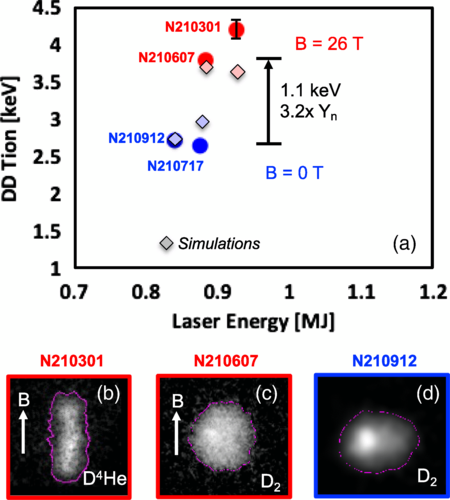
\includegraphics[width=0.5\linewidth]{Results2/Images/magnif_yield_inc.png}
    \centering
    \caption{a) A 1.1 keV $T_i$ increase was achieved by adding a 26 T $B_0$ field to a D${}_{2}$ gas capsule implosion on the \ac{NIF}.
    Also shown in the plot are the simulation results.
    b)$\rightarrow$d) Equatorial shapes of the implosions.
    Reused with permission from Ref.~\cite{moody_increased_2022}.}%
    \label{fig:Res2_moody_magnif}
\end{figure}

Indirect-drive experiments have been conducted on the \ac{NIF} to demonstrate the efficacy of magnetised targets, in reducing thermal conduction losses in the hotspot.
Non-cryogenic, deuterium filled capsules were deployed with initial field strengths up to $26\ \text{T}$~\cite{moody_increased_2022}.
Results from this experimental campaign are show in Fig.~\ref{fig:Res2_moody_magnif}.a.
Fig.~\ref{fig:Res2_moody_magnif}.b,~\ref{fig:Res2_moody_magnif}.c and ~\ref{fig:Res2_moody_magnif}.d plot x-ray images at stagnation of different experiments, showing that a shape-tuning process had to be conducted in order to optimise the sphericity of the target, due to the field leading to anisotropic thermal conduction.
The magnetised targets demonstrated significantly enhanced ion temperatures and neutron yields and work is underway to explore non-uniform field configurations to further enhance the benefits of magnetisation~\cite{walsh_application_2023}.

\begin{figure}[t!]
    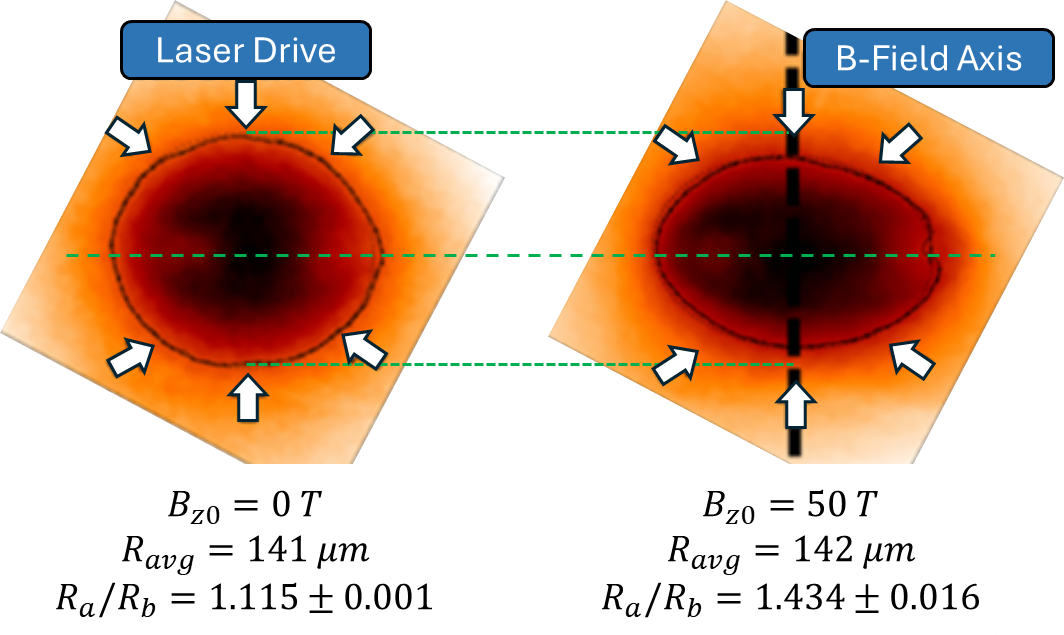
\includegraphics[width=0.6\linewidth]{Results2/Images/MagP2_Bose.png}
    \centering
    \caption{X-ray self emission images of (left) an unmagnetised and (right) a magnetised implosion.
    The average radius of the marked contour (corresponding to 40\% of peak intensity), and the oblateness parameter $R_a/R_b$ (ratio of major-to-minor axis) are listed below each image.
    The polar laser-drive is indicated by the white arrows, and the axis of the initial magnetic field by the black dashed line on the right.
    Applying an initial magnetic field demonstrated increased oblateness of the implosion.
    Adapted with permission from Ref.~\cite{bose_effect_2022}.}%
    \label{fig:Res2_Bose_magp2}
\end{figure}

Magnetisation of direct-drive targets has been investigated by experiments on the \textsc{Omega} laser facility for a number of years.
Initial \textsc{Omega} experiments focussed on verification of magnetic flux compression, by applying an initial seed field along the axis of a cylinder that was imploded via laser irradiation~\cite{gotchev_laser-driven_2009}.
The magnetised implosions validated predictions of flux compression and demonstrated enhanced neutron yields and core ion temperautres over unmagnetised implosions.
Spherical targets were subsequently fielded, which also resulted in increased stagnation temperatures and yield compared to unmagnetised targets.
No noticeable degradation to the implosion shape or performance was observed in these experiments, which was assumed to be due to the high ratio of plasma pressure to magnetic pressure, $\beta\gg 1$.

The most recent experimental, magnetised direct-drive work has focussed on exploring higher initial seed field values ($|\vec{B}_0|\sim50\ \text{T}$ compared to $|\vec{B}_0|\sim8\ \text{T}$), to understand the saturation of performance with increasing field.
A shock-driven, exploding pusher target configuration was used for these experiments, in order to create high ion temperatures and thus create a platform to study magnetisated ions.
Exploding pushers are significantly different implosions compared to hot-spot ignition targets discussed in previous chapters and shall be described in detail in Sec.~\ref{sec:Res2_expl}.
Creating these strong fields at the target necessitated reducing the radius of the equatorial field coil compared to previous experiments, and therefore a 40-beam configuration had to be used, without the 20 equatorial beams, leading to a pole heavy laser drive.
The high fields of these implosions led to strongly magnetised coronal electrons, $\omega_e\tau_e\sim50$, resulting in strongly anisotropic thermal conduction $\kappa_{\perp,e}/\kappa_{\parallel,e}\sim10^{-4}$.
This is compared to previous experiments which produced $\omega_e\tau_e\sim1$ and therefore $\kappa_{\perp,e}/\kappa_{\parallel,e}\sim1/3$.
In direct-drive on \textsc{Omega}, laser deposition is transported to the ablation surface by electron thermal conduction, thus large electron Hall parameters led to an effective asymmetry of the implosion drive.

Fig.~\ref{fig:Res2_Bose_magp2} shows x-ray self-emission images of an unmagnetised (left) and magnetised (right) target with an initial $|\vec{B}_0|=50\ \text{T}$ seed field.
The strongly magnetised coronal electrons led to decreased drive $\perp\hat{\vec{B_0}}$, markedly increasing the oblateness of the diagnostic image compared to the unmagnetised target.
An ion magnetisation of $\omega_i\tau_i\sim7$ was also reported.
Previous \ac{Rad-MHD} modelling of these experiments, using the \textsc{Chimera} code, did not include the effects of \ac{CBET}.
The development of \textsc{Solas}, and particularly the \ac{CBET} model, motivated further computational study of these experiments, to explore whether \ac{CBET} played a significant role in dictating the shape of these implosions.
This is because \ac{CBET} is known to markedly compensate global, $\ell=1$ asymmetries~\cite{anderson_effect_2020,colaitis_inverse_2021}, therefore the anisotropy introduced from magnetisation could effect the action of \ac{CBET}.

%################################################################################
%################################################################################
\subsection{Magnetised Laser-Plasma Instabilities}%
\label{sec:Res2_maglpis}

Some of the work conducted in this chapter, aims to understand how magnetisation of a direct drive implosion anisotropically changes the hydrodyanmics, and how these altered coronal plasma conditions modify the calculated \ac{CBET} gains, discussed in Sec.~\ref{sec:SOLAS_ray_power_change}.
For example, magnetisation restricts thermal conduction and therefore enhances coronal elecron temperatures along the initial field axis.
Approximately, the fluid \ac{CBET} gain, $\gamma_{ij}\propto T_e^{-1}$, therefore anisotropic changes to $T_e$ could result in reduced \ac{CBET} gains around the target and therefore change \ac{CBET} scattering compared to implosions without an applied field.
This modification to \ac{CBET} via the altered hydrodynamic profiles is called the \textit{indirect} effect of magnetisation on \ac{LPIs}.

Magnetisation can however also \textit{directly} modify scattering from \ac{LPIs}, in a number of ways.
For \ac{ICF} conditions, when the field strength is sufficently high, electron cyclotron motion can become comparable to plasma wave frequencies, and therefore alter the dispersion relation of the mediating plasma wave in \ac{LPIs}.
In underdense, \ac{ICF} relevant plasma ($n_e\sim 10^{20}\ \text{cm}^{-3}$ and $T\sim2\ \text{keV}$), the ion accoustic wave, which mediates \ac{SBS} and \ac{CBET}, is significantly modified when $|\vec{B}|\sim100\ \text{T}$ and the \ac{EPW}, which mediates ac{SRS} and \ac{TPD}, when $|\vec{B}|\sim1000\ \text{T}$~\cite{shi_benchmarking_2023}.
Additionally, the (predominnantly collisionless) damping of plasma waves can also be modified, because cylclotron motion of particles can affect their trapping in plasma waves~\cite{shi_benchmarking_2023}.
Significant theoretical progress has been made in this field in recent years by Shi \text{et al.}, who derived analytic formula for 3 wave coupling in the presence of a magnetic field \cite{shi_three-wave_2017,shi_laser-plasma_2018}.
This was challenging due to the lack of simple geometries for the interaction, when a field is applied to a plasma with an arbitrary direction.

The simulation results here neglect this direct affect of magnetisation on \ac{CBET}, partially because the theory is not yet deemed to be significantly mature, to implement within a reduced, ray-based model.
Coronal magnetic field strengths of $|\vec{B}|\lesssim50\ \text{T}$ were observed in the underdense coronal plasma so significant modifications to the accoustic wave dispersion relation were not expected.
It is noted however, that altered damping of the waves from magnetisation may affect the results, but the focus of the study was predominantly to explore how magnetisation might indirectly affect \ac{CBET}.

%################################################################################
%################################################################################
\subsection{The Exploding-Pusher Configuration}%
\label{sec:Res2_expl}

Exploding-pushers are considered to be a highly reproducible platform, robust to instabilities and capable of producing large neutron yields.
Although historically it had a slightly different meaning~\cite{craxton_direct-drive_2015}, the term `exploding pusher' is now, typically used for low convergence, thin-shell targets~\cite{ellison_development_2018}.
When irradiated with significant intensity, frequency-tripled laser light\footnote{When frequency-tripled light is not used, suprathermal electrons, rather than ablation, is the dominant driver of the strong shock~\cite{yeamans_high_2021}.}, the thin shell rapidly heats and then explosively ablates, driving a strong shock radially inward, ahead of the in-falling ablated material.
This shock strongly heats the ions as it propagates through gas fill to large, fusion relevant temperatures.
After rebounding from the axis, the shock recompresses the infalling exploded shell material, resulting in sufficient density for a significant number of fusion reactions.

Directly-driven exploding pusher targets have the largest direct drive fusion yields recorded on the \ac{NIF}, resulting in $E_{\text{fusion}}\sim 30\ \text{kJ}$~\cite{yeamans_high_2021}.
However, they are not suitbale for high gain designs, as the low areal densities of the target are not sufficient to confine $\alpha$ particles and thus enable burn propagation.
A variety of interesting physics may be studied using the platform due to the significant ion temperatures that can be achieved, such as equilibration between electrons and ions~\cite{benedict_molecular_2012}.
The strong shock is also highly kinetic, and thus accurate comparison to experimentally measureable variables, such as yields and ion temperatures, is expected to be difficult for \ac{Rad-Hydro} codes which lack a suitbale model for non-local transport, such as \textsc{Chimera}.
However, much of the key dynamics and serults can be studied more qualitatively.
!!!!!!!!!!!!!!!!!!!!!!!!!!!!! - Check tha above sentance and get a reference - !!!!!!!!!!!!!!!!!!!!!!!!!!!!!!!!!!!!!!!!!

%###############################################################################################################################
%###############################################################################################################################
%###############################################################################################################################
\section{Effect of Cross-Beam Energy Transfer in Unmagnetised Exploding Pushers}%
\label{sec:Res2_CBET_expl}

This section presents simulation results of the effect of \ac{CBET} in exploding pushers on \textsc{Omega}.
Both 1-D and 2-D \textsc{Chimera}-\textsc{Solas} simulations of 40-beam, polar driven exploding pusher experiments are presented, with a focus on how \ac{CBET} acts to change the implosion.
The 1-D results demonstrate that \ac{CBET} significantly reduces the coupled laser energy to the implosion from \dots to \dots.
Simulations conducted in 2-D, with a full 3-D raytrace and \ac{CBET} model, show that \ac{CBET} alters spatial profile of the laser deposition, reducing asymmetry in the drive.



%################################################################################
%################################################################################
\subsection{Simulation Configuration}%
\label{sec:Res2_simconfig}


\begin{figure}[t!]
    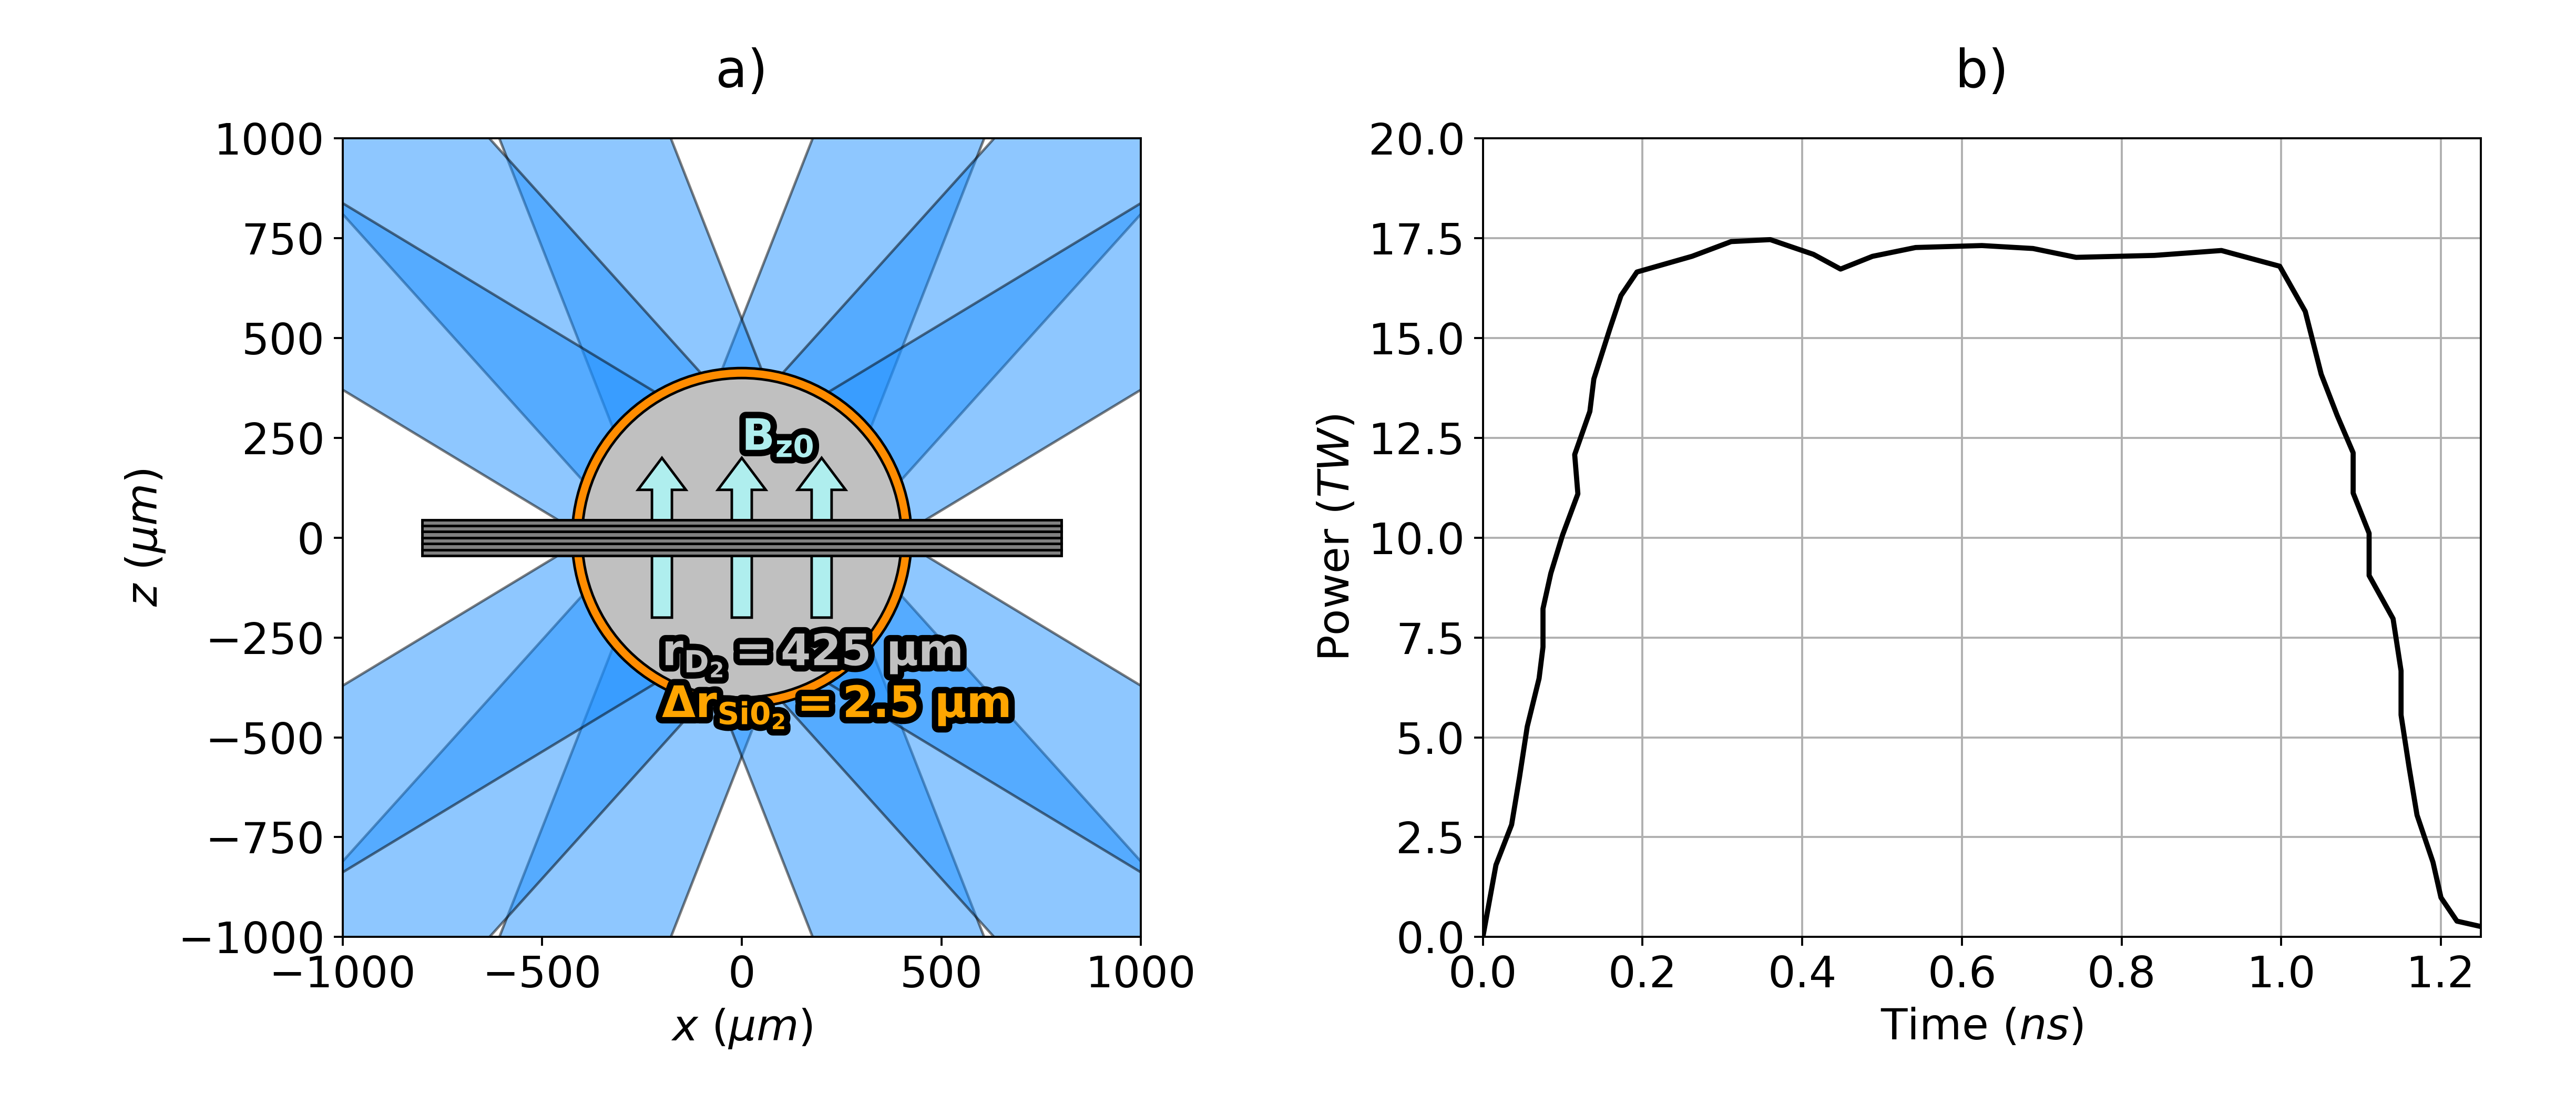
\includegraphics[width=\linewidth]{Results2/Images/magpdd_diagram_pulse.png}
    \centering
    \caption{The initial conditions used for all simulations presented in this chapter.
    Panel a) plots the D${}_{2}$ filled, glass shell capsule and direction of the initial magnetic field.
    An example field coil (illustrative and not included in simulations) is also shown, the presence of which necessitated the polar laser drive in experiments.
    Panel b) plots the laser pulse shape used, which had a total of $17.7\ \text{kJ}$ laser energy.}%
    \label{fig:Res2_simconfig}
\end{figure}


%################################################################################
%################################################################################
\subsection{1-D Simulations}%
\label{sec:Res2_expl1D}

\bgroup%
\def\arraystretch{1.3}%  1 is the default, change whatever you need
% Please add the following required packages to your document preamble:
% \usepackage{multirow}
\begin{table}[]
    \centering
    \caption{Results of all Simulations. In the \ac{CBET} column, `$\sim$' indicates \ac{CBET} acted on the magnitude, but \textit{not} spatial location, of deposition.}
    \begin{tabular}{cccccccccc}
        \hhline{==========}
        Run & Dim. & CBET   & Note      & \begin{tabular}[c]{@{}c@{}}$B_{z0}$\\ $(\mathrm{T})$\end{tabular} & \begin{tabular}[c]{@{}c@{}}$t_b$\\ $(\mathrm{ns})$\end{tabular} & \begin{tabular}[c]{@{}c@{}}$\langle T_i \rangle$\\ (keV)\end{tabular} & \begin{tabular}[c]{@{}c@{}}$Y_n$\\ $(\times10^{10})$\end{tabular} & \begin{tabular}[c]{@{}c@{}}$\Delta_b$\\ (ps)\end{tabular} & $\frac{R_{\text{equator}}}{R_{\text{pole}}}\bigg|_{t=t_b}$              \\ \hline
        1   & 1-D  & Off    & -         & 0                                                                 & 0.69                                                            & 14.66                                                                 & 11.62                                                            & 87                                                        & $1.00_{-0.00}^{+0.00}$ \\
        2   & 1-D  & On     & -         & 0                                                                 &                                                                 &                                                                       &                                                                  &                                                           & $1.00_{-0.00}^{+0.00}$ \\
        3   & 2-D  & Off    & -         & 0                                                                 & 0.71                                                            & 8.44                                                                  & 6.20                                                             & 148                                                       & $2.96_{-0.19}^{+0.20}$ \\
        4   & 2-D  & $\sim$ & -         & 0                                                                 & 0.75                                                            & 7.61                                                                  & 5.23                                                             & 153                                                       & $3.26_{-0.23}^{+0.25}$ \\
        5   & 2-D  & On     & -         & 0                                                                 & 0.75                                                            & 7.77                                                                  & 5.46                                                             & 148                                                       & $3.23_{-0.23}^{+0.25}$ \\
        6   & 2-D  & Off    & -         & 25                                                                & 0.74                                                            & 7.26                                                                  & 4.73                                                             & 130                                                       & $3.80_{-0.33}^{+0.41}$ \\
        7   & 2-D  & $\sim$ & -         & 25                                                                & 0.78                                                            & 6.58                                                                  & 4.14                                                             & 125                                                       & $4.55_{-0.43}^{+0.50}$ \\
        8   & 2-D  & On     & -         & 25                                                                & 0.78                                                            & 6.72                                                                  & 4.44                                                             & 123                                                       & $4.32_{-0.41}^{+0.47}$ \\
        9   & 2-D  & Off    & -         & 50                                                                & 0.73                                                            & 6.82                                                                  & 3.73                                                             & 134                                                       & $4.40_{-0.38}^{+0.43}$  \\
        10  & 2-D  & $\sim$ & -         & 50                                                                & 0.78                                                            & 6.30                                                                  & 3.30                                                             & 130                                                       & $4.92_{-0.48}^{+0.56}$  \\
        11  & 2-D  & On     & -         & 50                                                                & 0.78                                                            & 6.37                                                                  & 3.52                                                             & 129                                                       & $4.79_{-0.47}^{+0.55}$ \\
        12  & 2-D  & Off    & No Aniso. & 25                                                                & 0.81                                                            & 6.40                                                                  & 5.02                                                             & 118                                                       & $3.14_{-0.50}^{+0.68}$ \\
        13  & 2-D  & Off    & No Lor.   & 25                                                                & 0.74                                                            & 7.29                                                                  & 4.77                                                             & 131                                                       & $3.80_{-0.33}^{+0.41}$ \\
        14  & 2-D  & Off    & No Nern.  & 25                                                                & 0.73                                                            & 7.41                                                                  & 4.85                                                             & 130                                                       & $3.74_{-0.32}^{+0.38}$ \\
        15  & 2-D  & Off    & No Resis. & 25                                                                & 0.73                                                            & 7.07                                                                  & 4.59                                                             & 132                                                       & $3.84_{-0.33}^{+0.42}$ \\ \hhline{==========}
\end{tabular}
\end{table}
\egroup%


\begin{figure}[t!]
    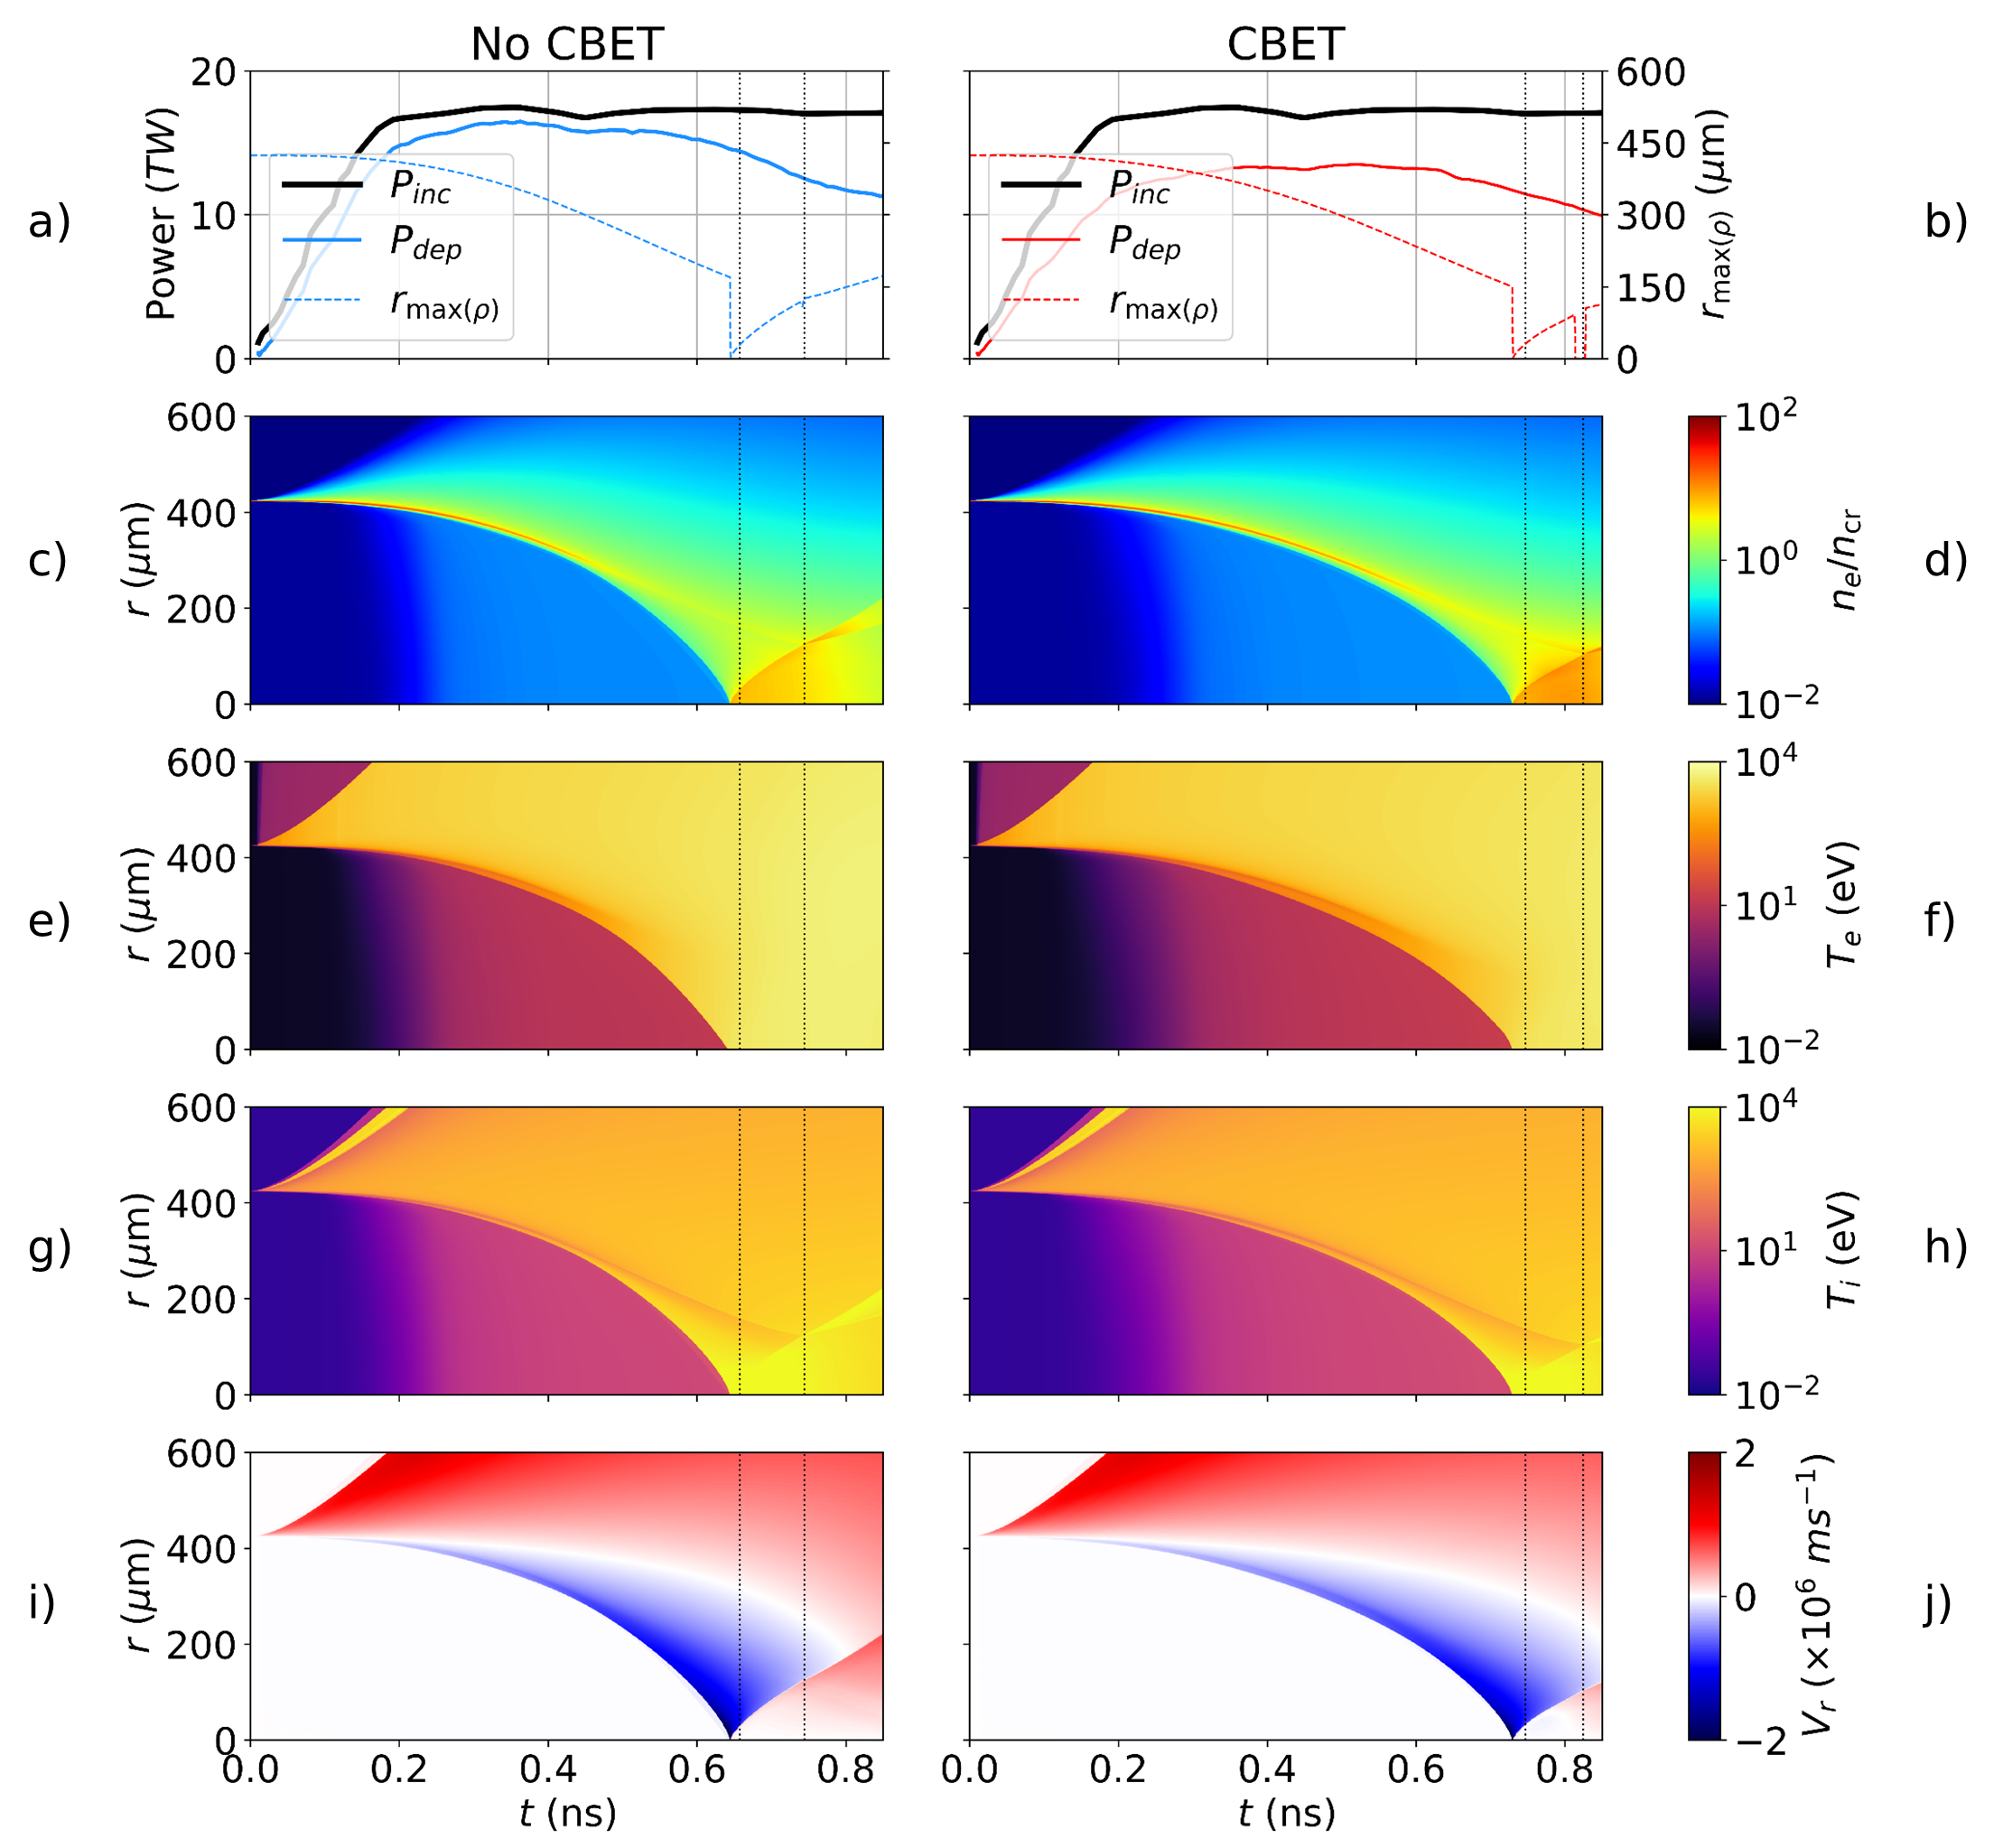
\includegraphics[width=\linewidth]{Results2/Images/expl_streaks.png}
    \centering
    \caption{1-D Simulation results both without (left) and with (right) \ac{CBET}.
    The top row plots the incident and absorbed energy from the simulation on the left axis and the radius of maximum density on the right.
    In order, the next rows plot $n_e$, $T_e$, $T_i$ and $V_r$.
    The full-width half-maximum times of the D${}_{2}$ yield are plotted as dotted vertical black lines on all panels.}%
    \label{fig:Res2_expl_streaks}
\end{figure}

%################################################################################
%################################################################################
\subsection{2-D Simulations}%
\label{sec:Res2_expl2D}


\begin{figure}[t!]
    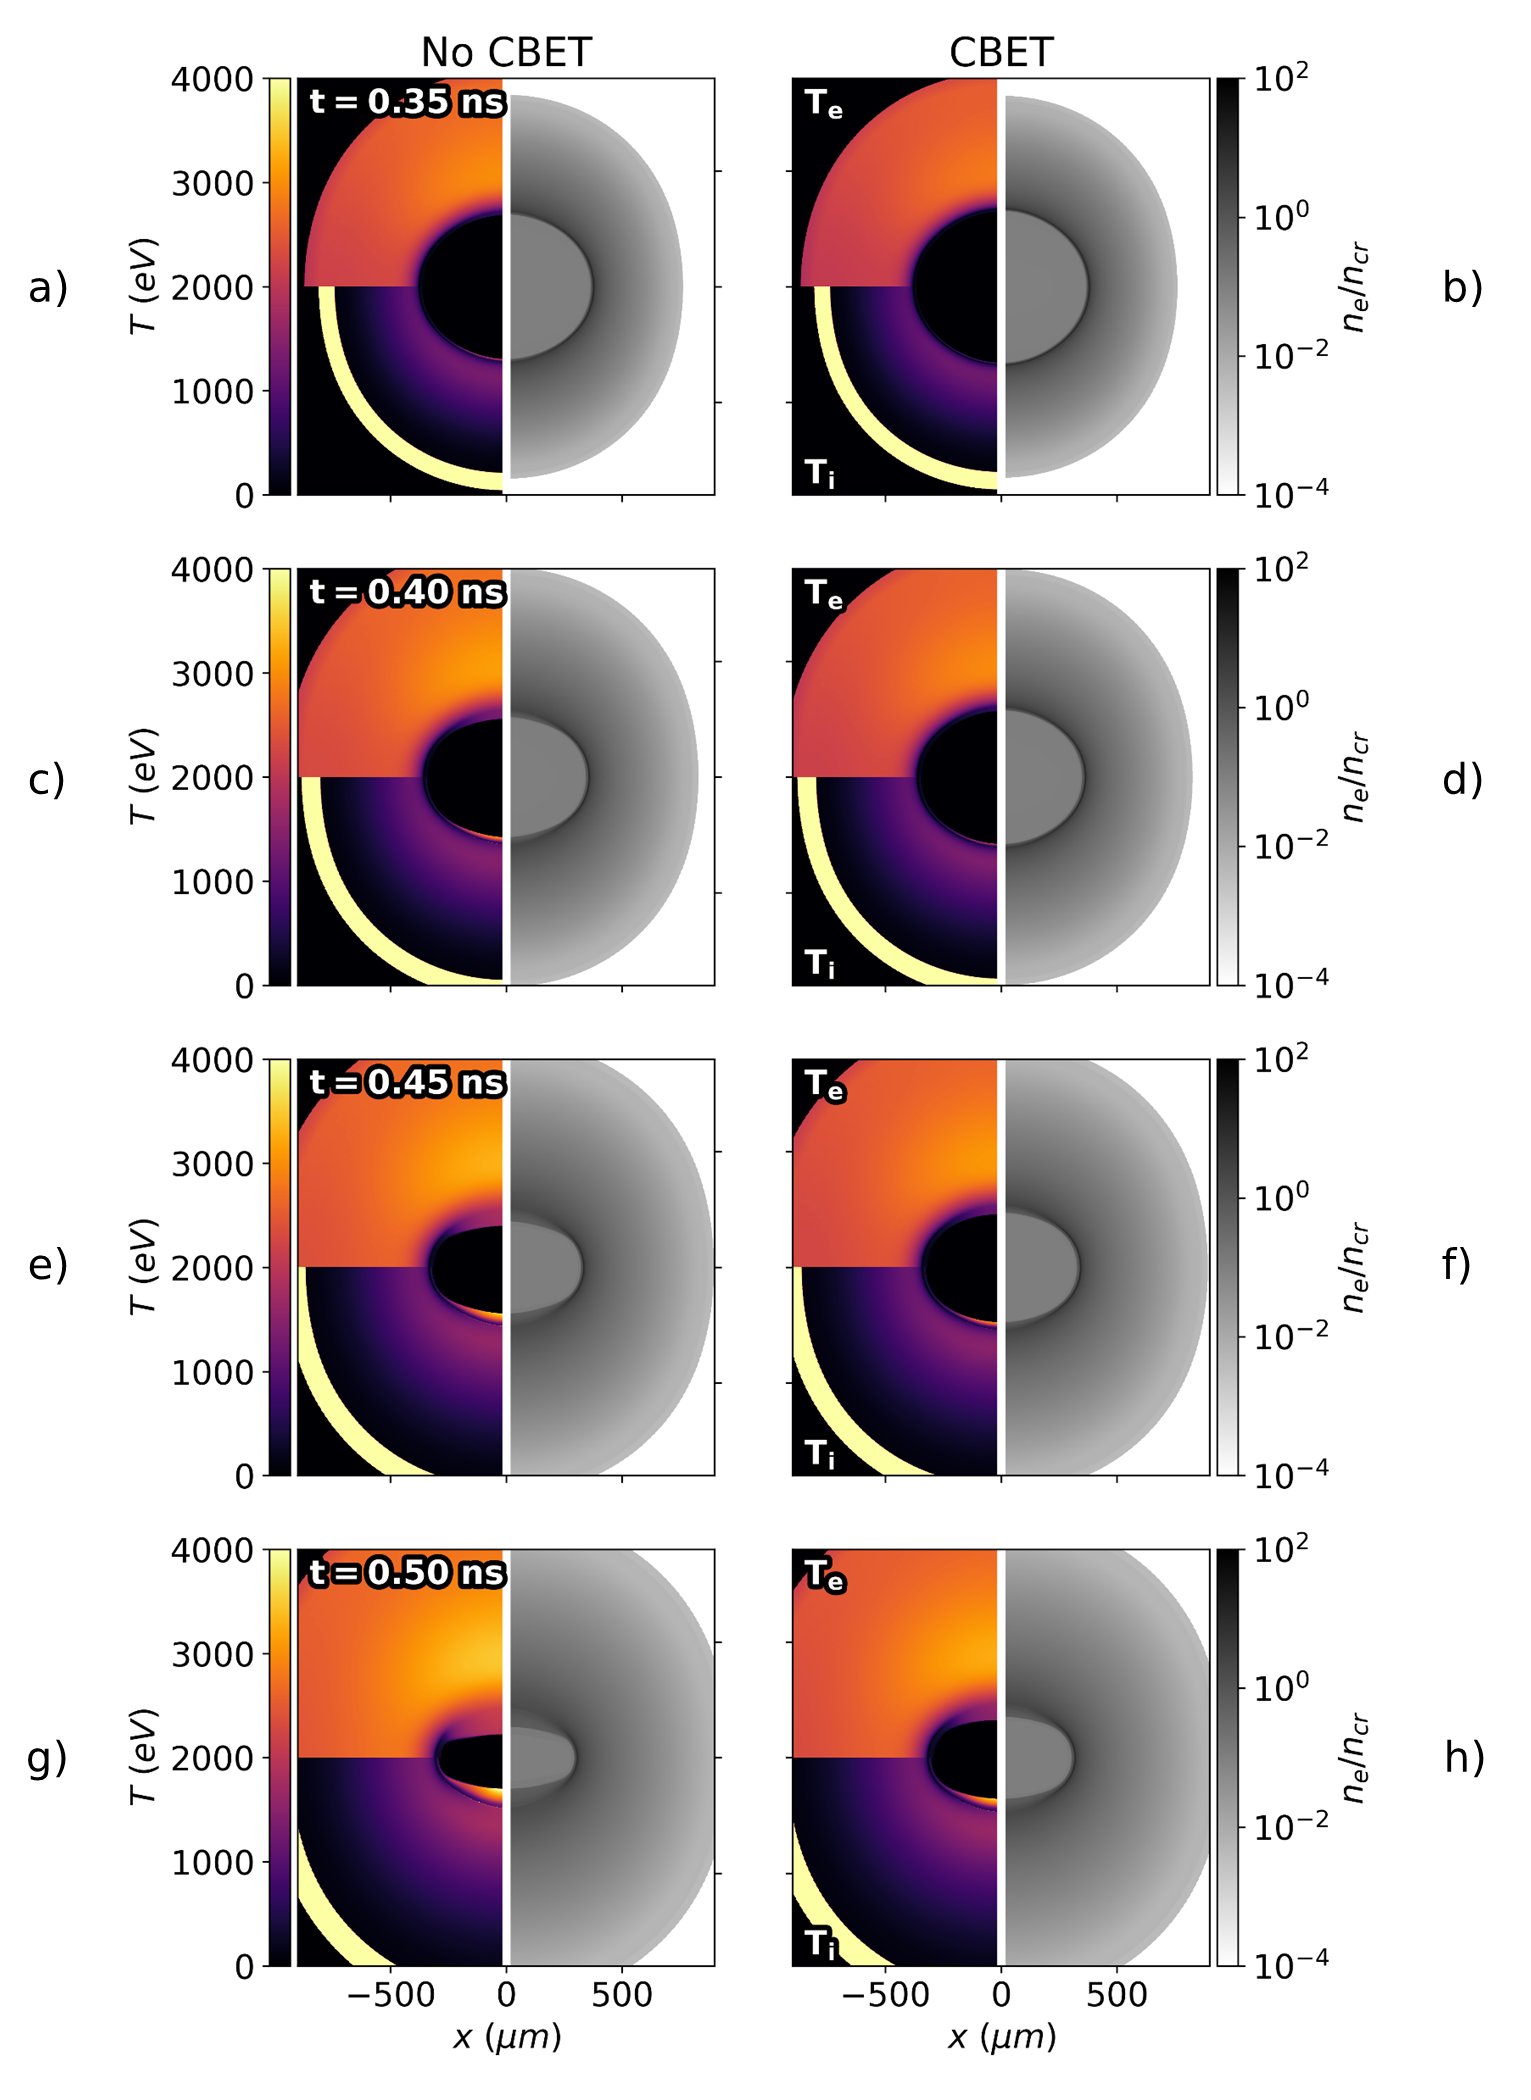
\includegraphics[width=0.95\linewidth]{Results2/Images/unmag_CBET_onoff.png}
    \centering
    \caption{$n_e$ (right-side), $T_e$ (top-left-side) and $T_i$ (bottom-left-side) plots from the 2-D, $0\ \text{T}$ simulations without (left) and with (right) \ac{CBET} at a variety of in-flight times.
    The decreased deposited energy due to \ac{CBET}, results in lower coronal electron temperatures and therefore a slower, weaker shock being driven, which is especially evident at later times.}%
    \label{fig:Res2_unmag_CBET_onoff}
\end{figure}



%###############################################################################################################################
%###############################################################################################################################
%###############################################################################################################################
\section{The Effect of Magnetisation on Exploding-Pusher Implosions}%
\label{sec:Res2_mag_unmag}

This section presents results of a study of the effect that extended-\ac{MHD} has on the 2-D exploding pusher simulations.
Simulations were conducted with varying initial magnetic field strengths and particular terms turned off and on to deduce what the important physical processes are.
Magnetised transport is important for both initial seed magnetic field implosions, resulting in large coronal Hall parameters and therefore significant anisotropy of the implosions.
The results demonstrate that (resistive diffusion and the Lorentz force have very little impact on the implosion physics, due to the bulk of the plasma being highly resistive and high-$\beta$ respectively)?????.
The Nernst advection of magnetic field ????????????????????


%################################################################################
%################################################################################
\subsection{In-Flight Field Structure}%
\label{sec:Res2_field_structure}


\begin{figure}[t!]
    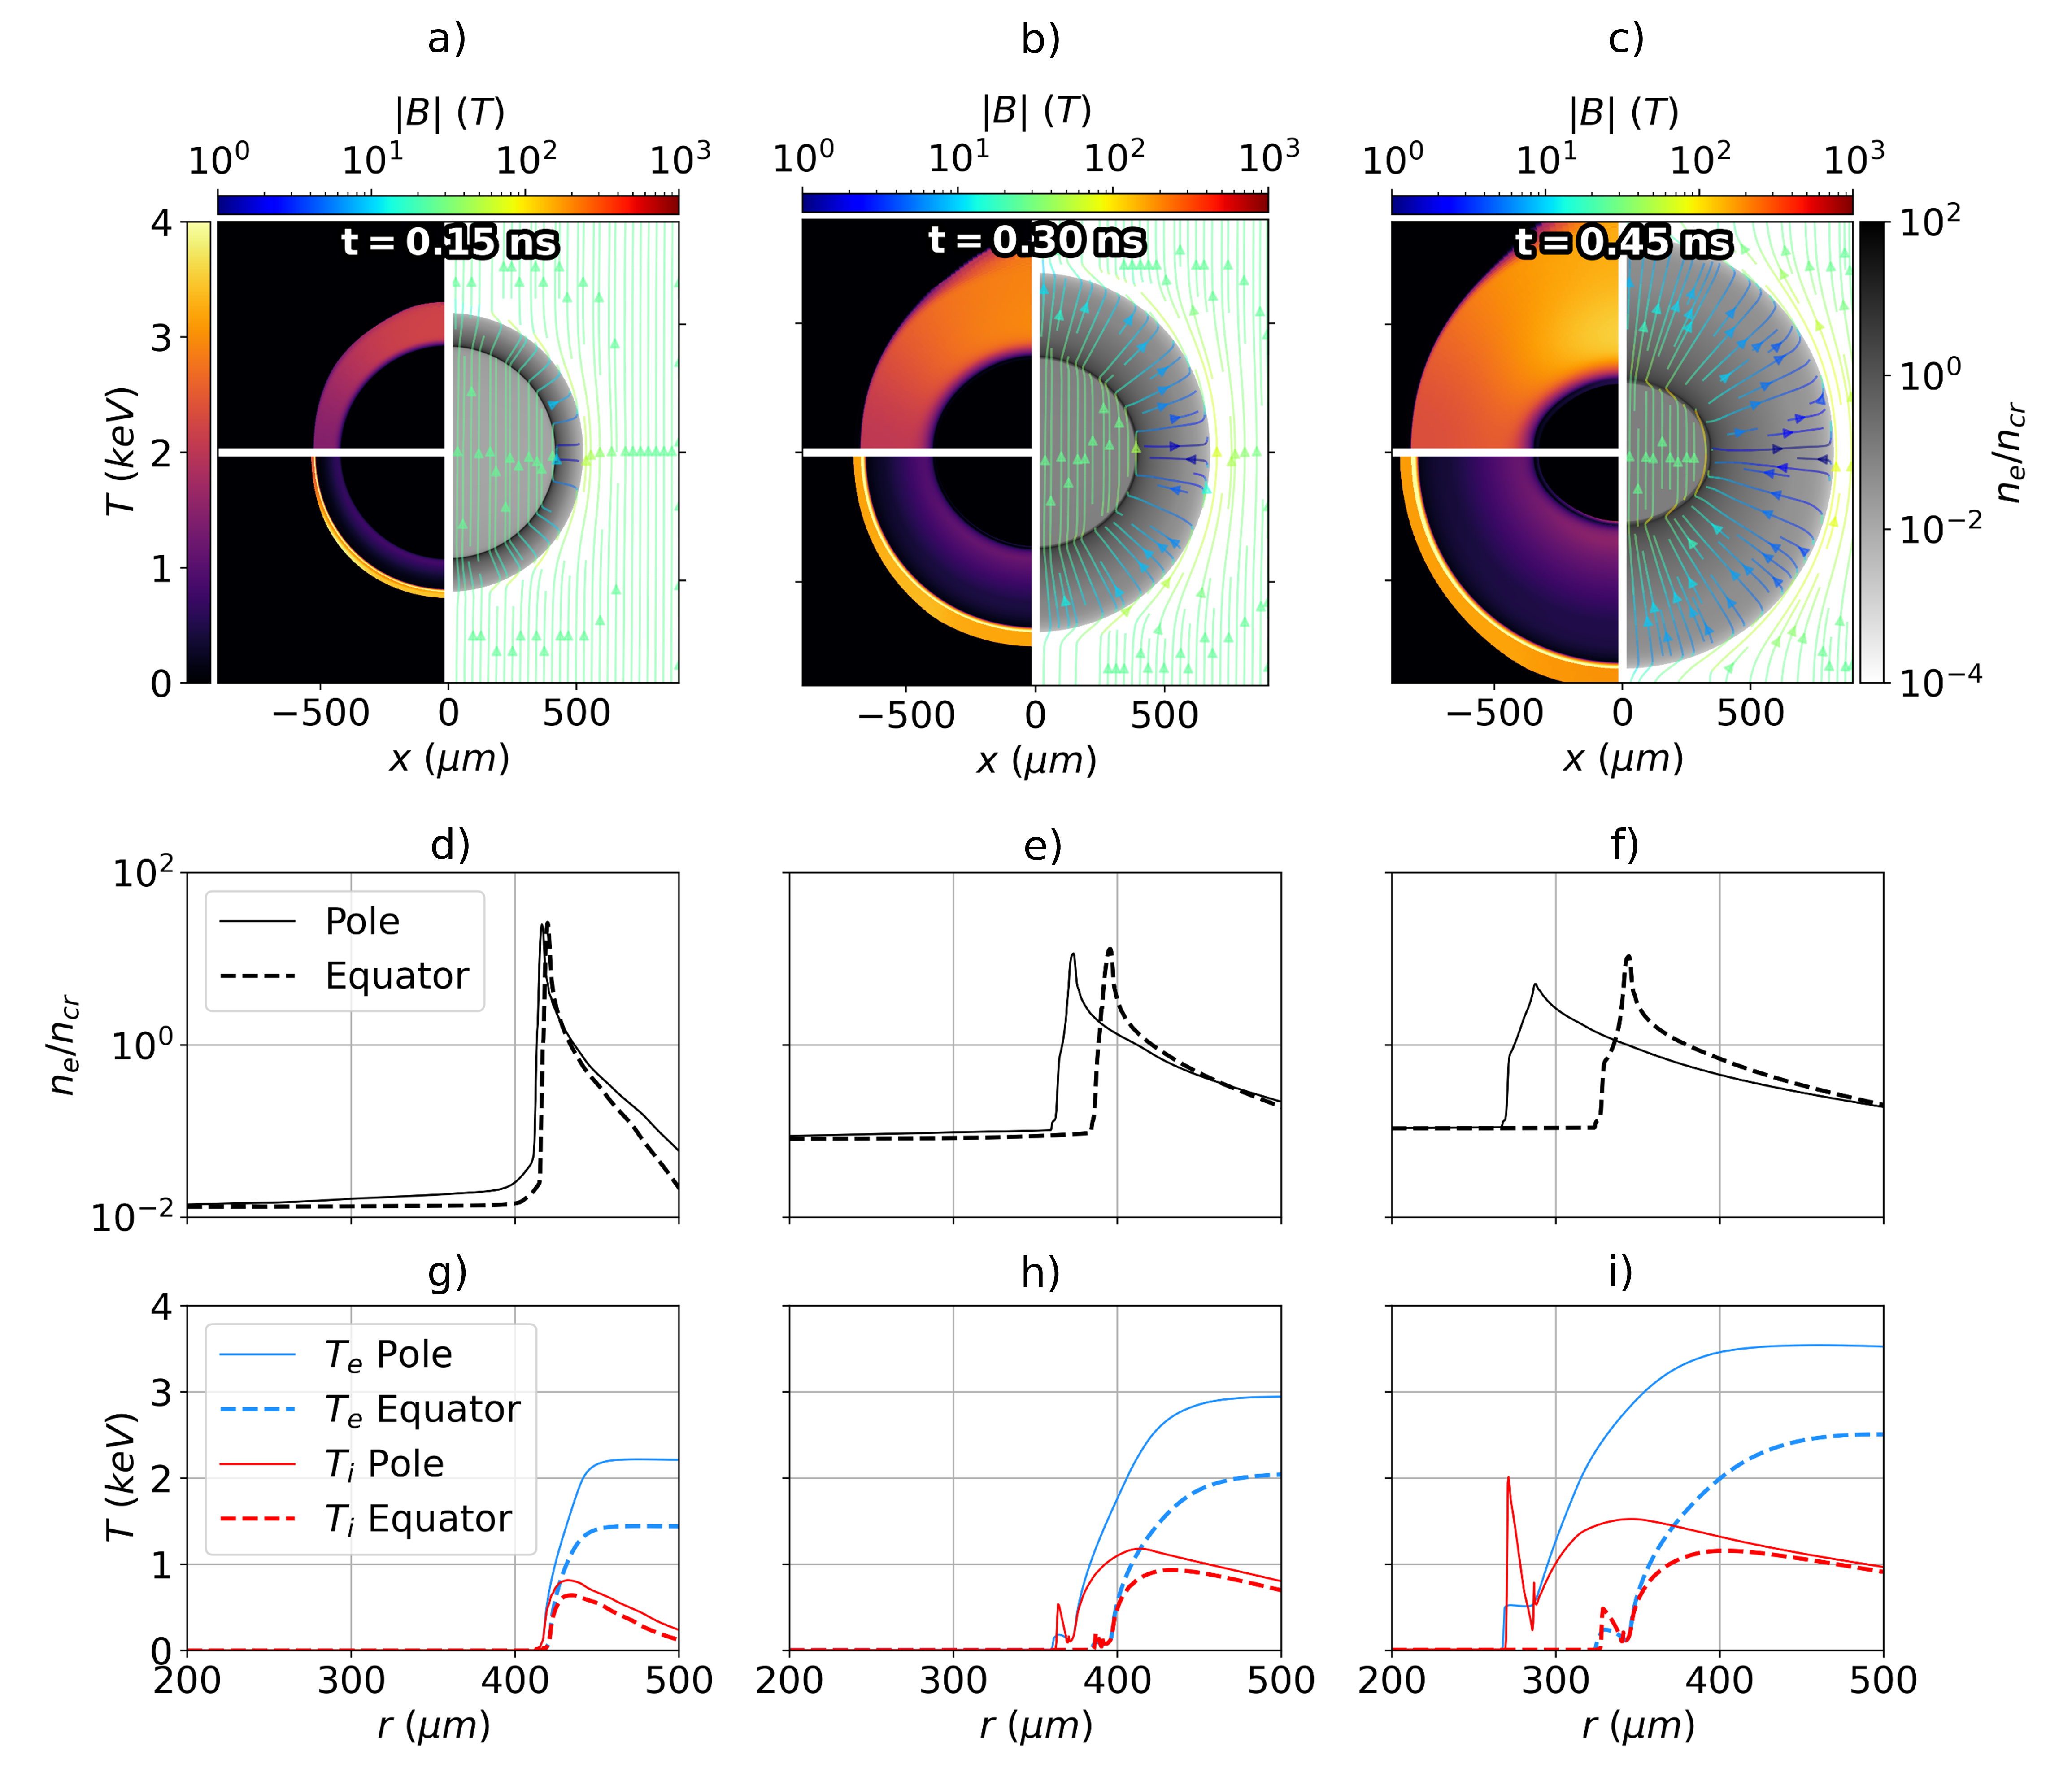
\includegraphics[width=\linewidth]{Results2/Images/mag_early_B_develop.png}
    \centering
    \caption{The development of the hydrodynamic variables and magnetic field structure from the $B_{z0}=25\ \text{T}$, \ac{CBET} simulation.
    Panels a), b) and c) plot $T_e$ (top-left), $T_i$ (bottom-left), $n_e$ (right) and $\vec{B}$ (streamlines) at $t=0.15$, $0.30$ and $0.45\ \text{ns}$ respectively.
    The approximately radially outward flowing, hot (and therefore highly conductive) ablating plasma pulls the magnetic field with it, resulting in radial $\vec{B}$ field lines, which are weaker at the capsule equator.
    The radial field lines in the corona prevent angular equilibration of temperature, so act to keep heat at the poles.
    Compression of the SiO${}_2$ shell leads to a non-radial field pile up on the inside edge of the maximum density, which is most clearly visible in panel c).
    Panels d), e) and f) plot $n_e$ lineouts along the pole ($\theta=0^{\circ}$) and equator ($\theta=90^{\circ}$).
    Panels g), h) and i) plot equivalent $T_e$ and $T_i$ lineouts.
    These all show that the increased polar temperatures, partially due to beam geometry and partially due to magnetisation, lead to preferential ablation at the pole.}%
    \label{fig:Res2_mag_early_B_develop}
\end{figure}



%################################################################################
%################################################################################
\subsection{Anisotropic Thermal Conduction}%
\label{sec:Res2_aniso}


\begin{figure}[t!]
    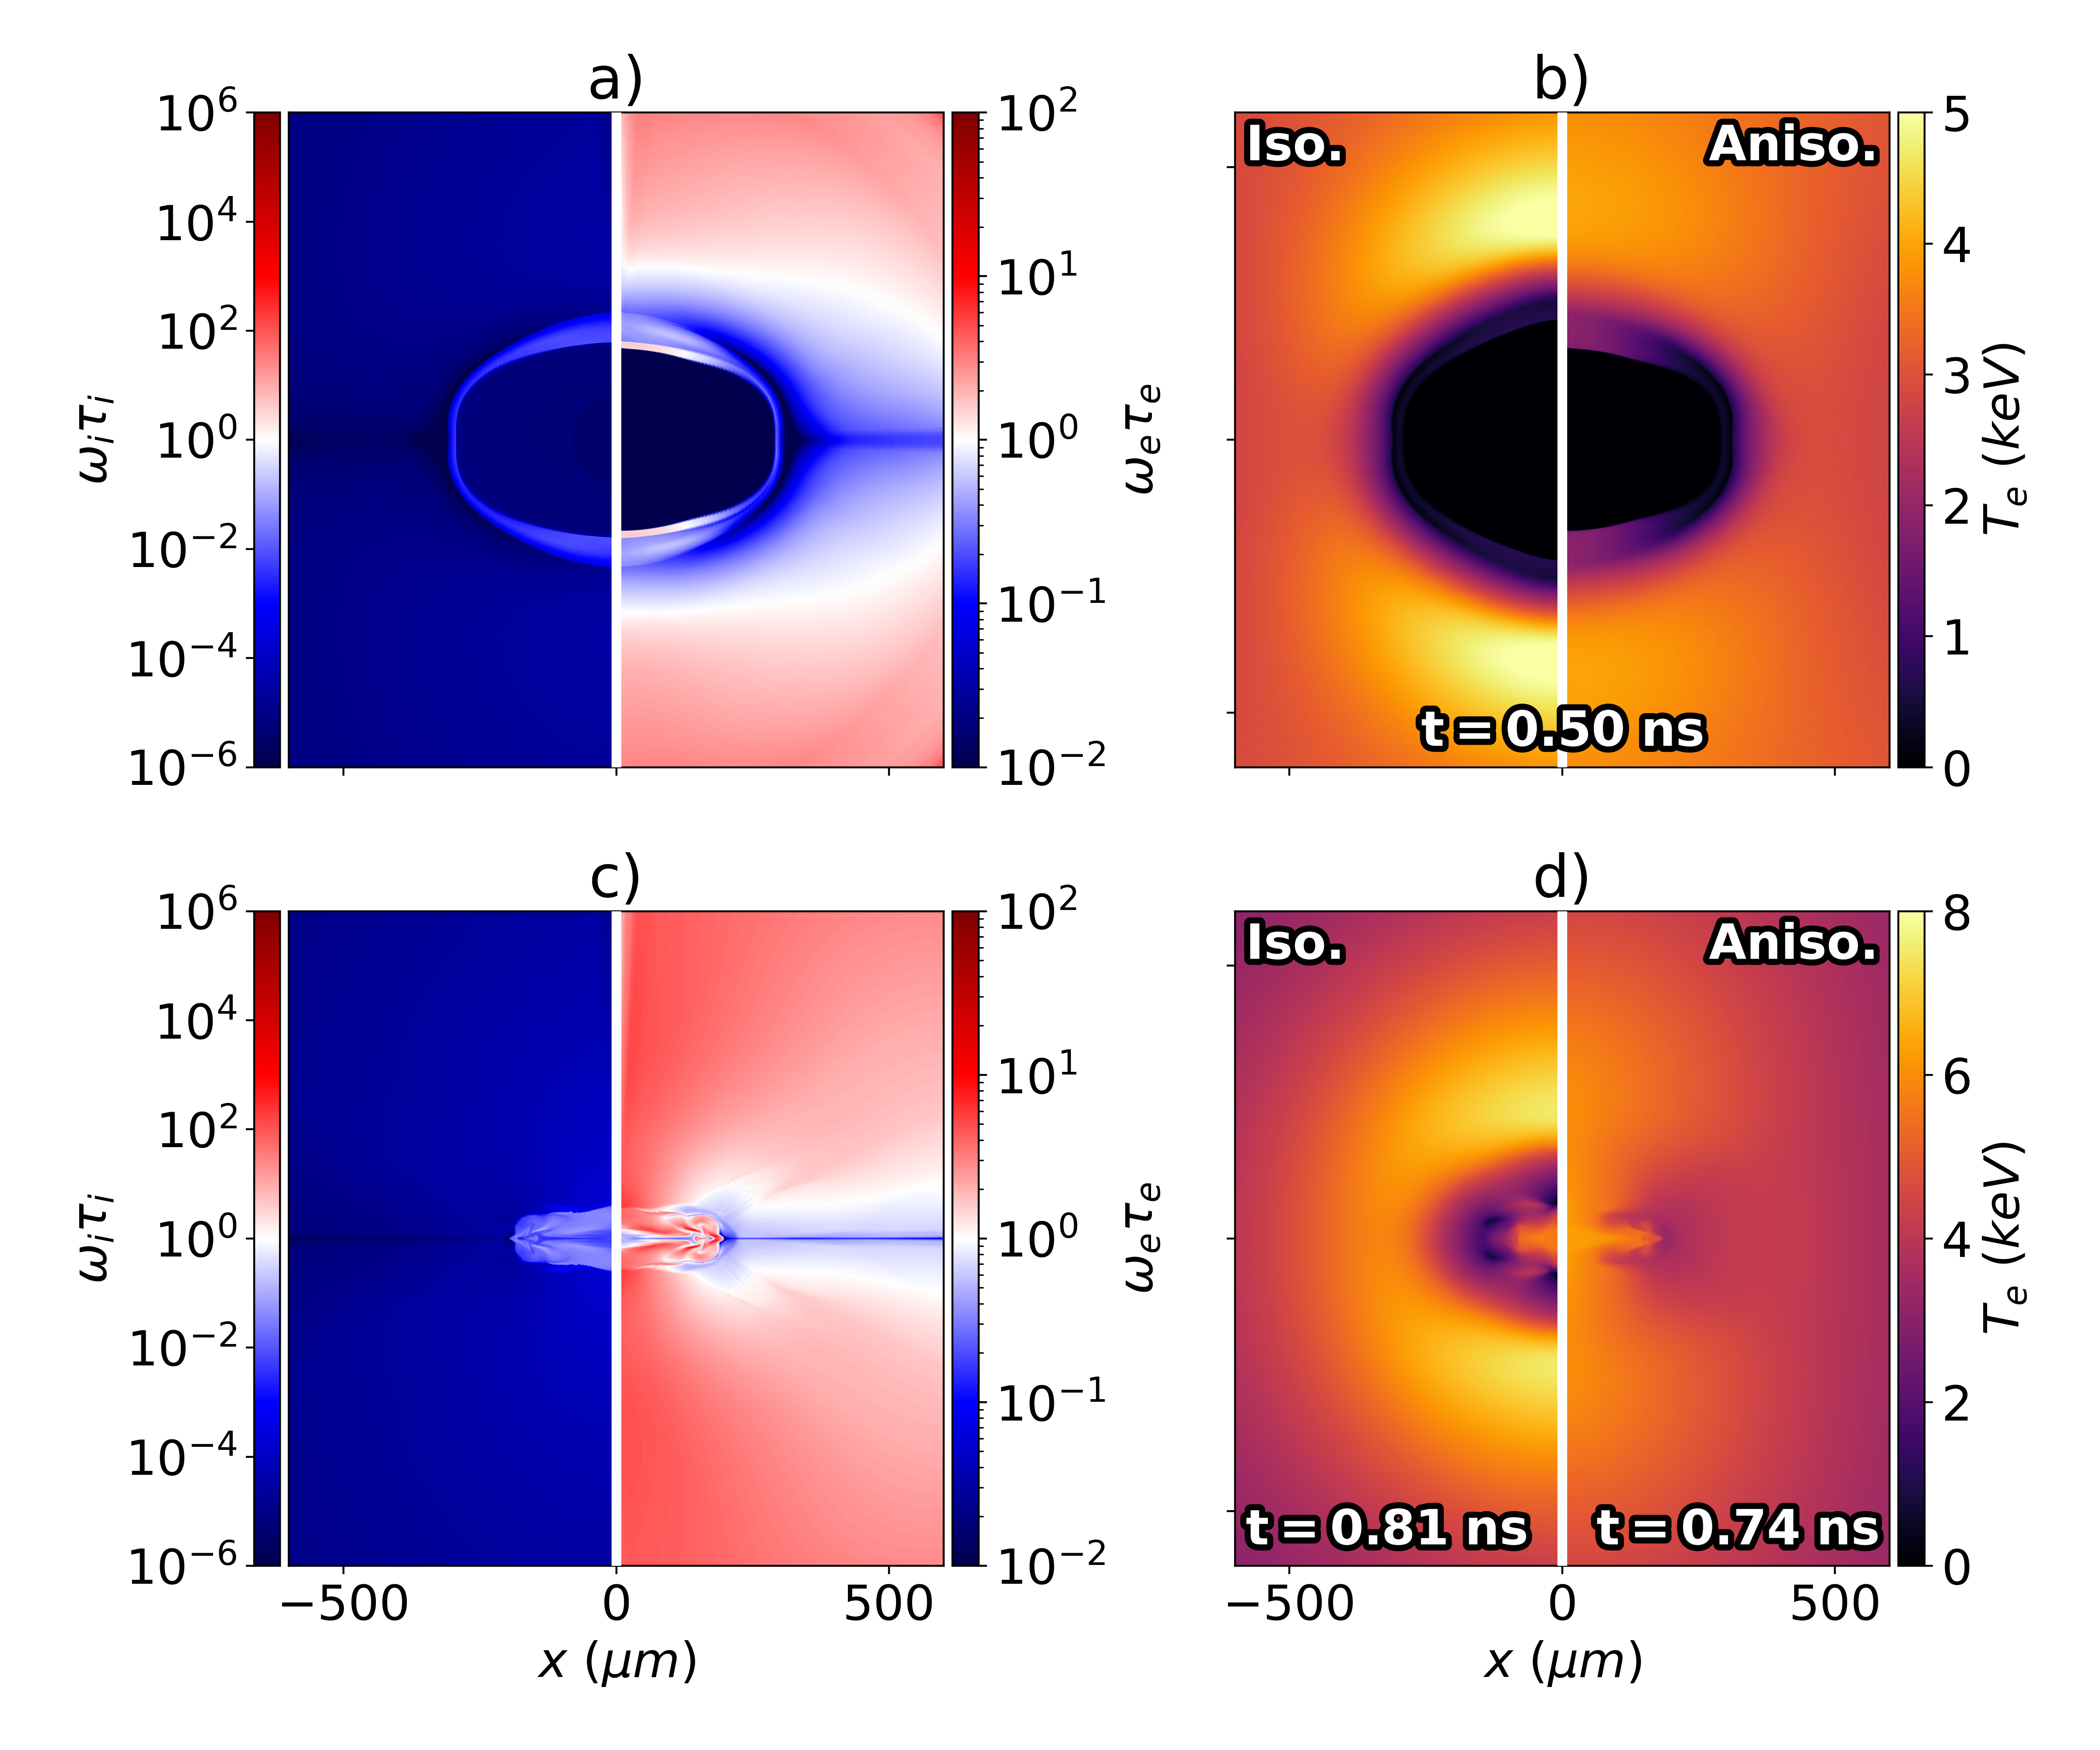
\includegraphics[width=0.8\linewidth]{Results2/Images/iso_aniso.png}
    \centering
    \caption{In-flight a) and bangtime c) Hall parameters, from the $B_{z0}=25\ \text{T}$, no-\ac{CBET}, anisotropic conduction simulation.
    Panel b) plots the $T_e$ from the isotropically magnetised simulation (left-side) and anisotropic conduction simulation (right-side) in-flight.
    Panel c) plots the $T_e$ from the isotropically magnetised simulation (left-side) and anisotropic conduction simulation (right-side) at peak neutron production.
    The electron Hall parameter is $>1$ at the poles due to high magnetic fields and temperatures, leading to significantly restricted thermal conduction from magnetised transport at the poles.
    Isotropically magnetised conduction (\textit{i.e.} setting $\kappa_{\parallel}=\kappa_{\perp})$, therefore results in a markedly different implosion morphology, as is shown in panels b) and d).
    Ion hall parameters peak at bangtime, with values reaching about $\omega_i\tau_i\sim0.1$.}%
    \label{fig:Res2_iso_aniso}
\end{figure}

%################################################################################
%################################################################################
\subsection{The Nernst Effect}%
\label{sec:Res2_nernst}


\begin{figure}[t!]
    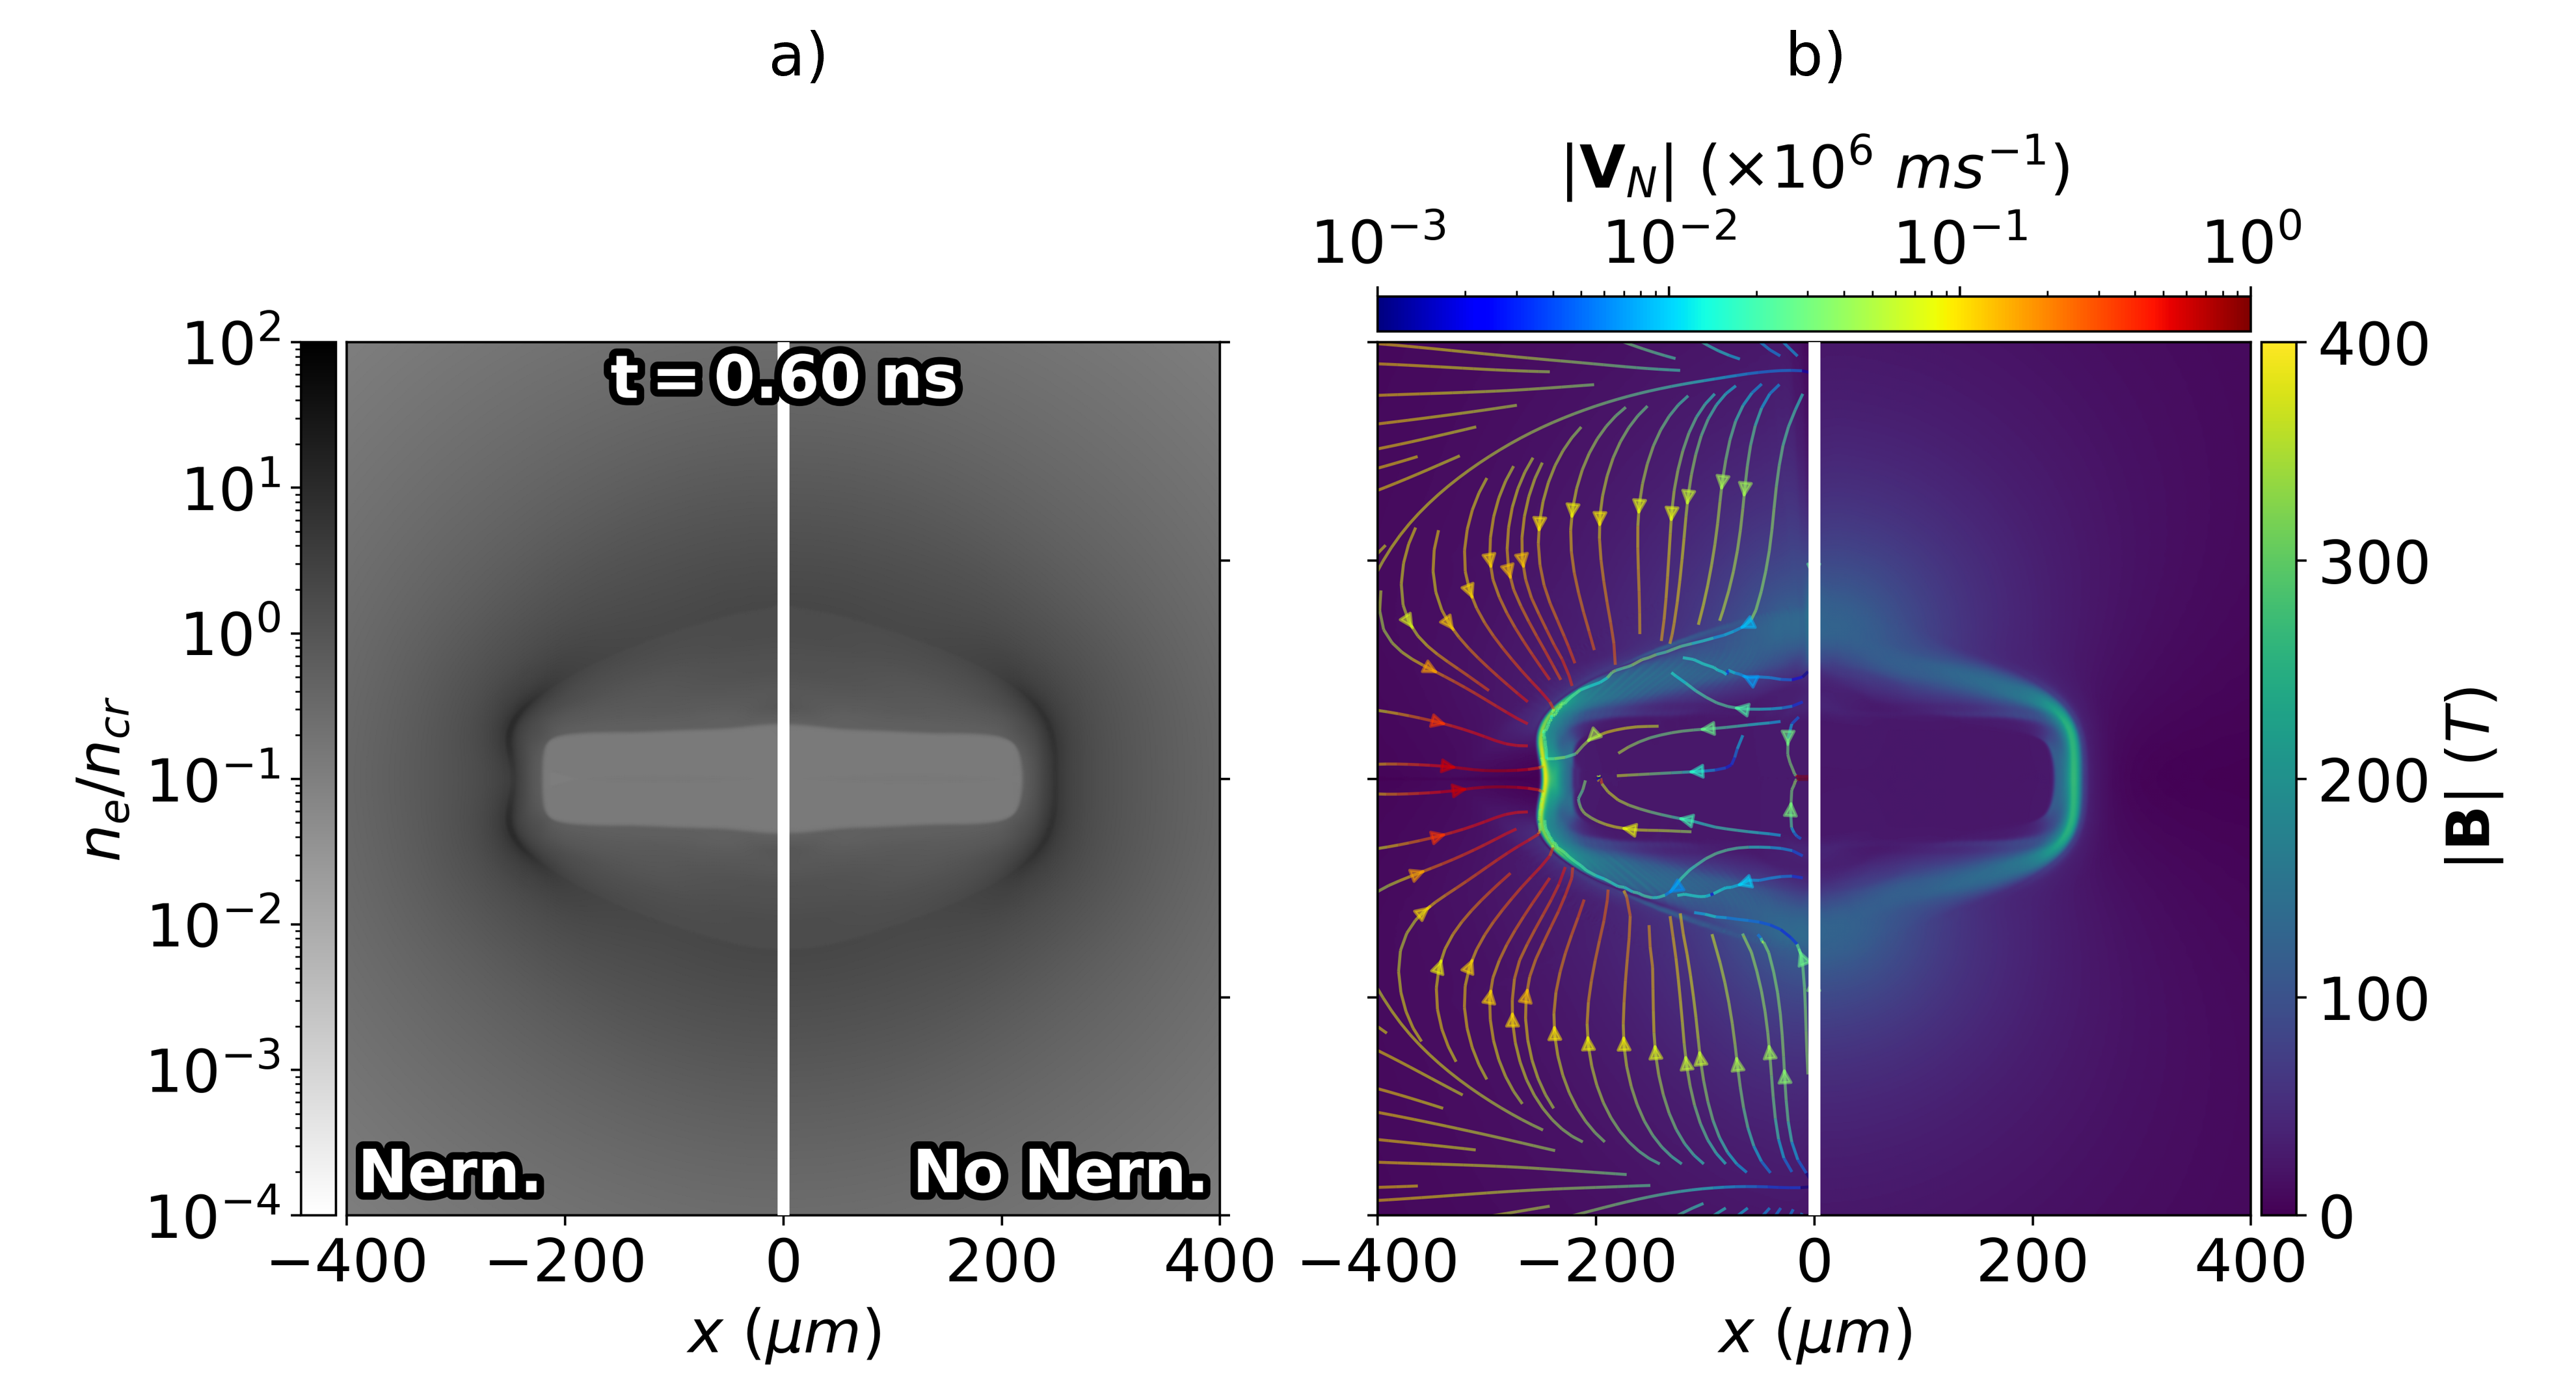
\includegraphics[width=0.8\linewidth]{Results2/Images/nernst_comp.png}
    \centering
    \caption{Panel a) plots in-flight electron density profiles from the $B_{z0}=25\ \text{T}$, no-\ac{CBET} simulations with (left-side) and without (right-side) Nernst advection of the magnetic field.
    Panel b) plots magnetic field magnitude from the Nernst (left-side) and no-Nernst (right-side) simulation.
    The Nernst advection velocity is also plotted for the Nernst simulation as streamlines, coloured by speed.
    Advection of the field is important in the low Hall parameter equatorial region, pulling $\vec{B}$ down $\nabla T_e$, into the dense wall.
    Altered field at the equator impacts on the magnetised thermal conduction, which ultimately imprints on the density, as is seen in panel a).}%
    \label{fig:Res2_nernst_comp}
\end{figure}



%################################################################################
%################################################################################
\subsection{Resistive Diffusion and the Lorentz Force}%
\label{sec:Res2_resis}

\begin{figure}[t!]
    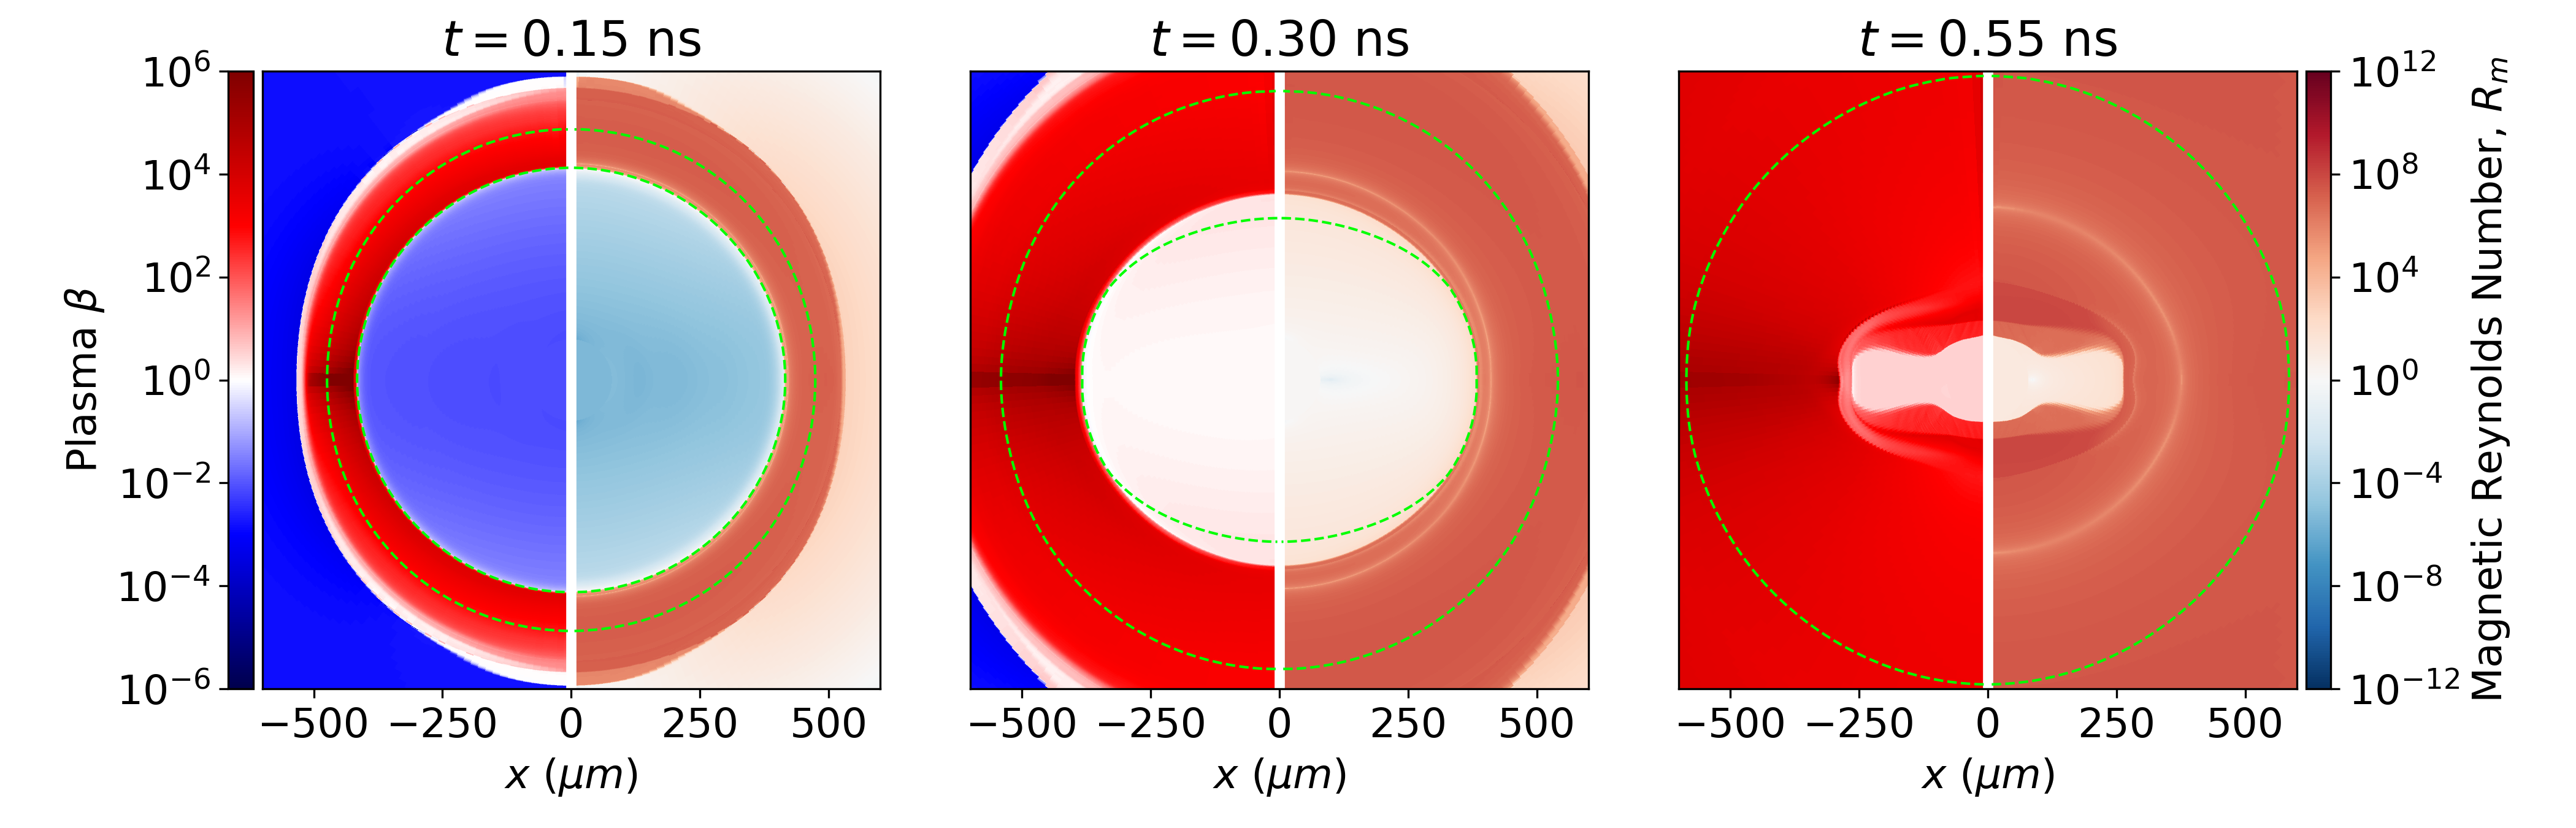
\includegraphics[width=\linewidth]{Results2/Images/magmag_beta_Rm.png}
    \centering
    \caption{Plasma $\beta$ (left-side) and Magnetic Reynolds Number, $R_m$, (right-side) at various in-flight times, throughout the $B_{z0}=25\ \text{T}$, no-\ac{CBET} simulation.
    Contours of the $n_e=n_{cr}/10$ are plotted on all panels as dashed green lines to indicate the bounding region containing a significant amount plasma.
    Broadly, the $\beta$ and $R_m$ values are $\gg 1$ in all regions with an appreciable amount of plasma, which demonstrate that the Lorentz force and resistive diffusion respectively, should have minimal effect on the implosion dynamics.}%
    \label{fig:Res2_magmag_beta_Rm}
\end{figure}



%###############################################################################################################################
%###############################################################################################################################
%###############################################################################################################################
\section{The Effect of Magnetisation on Cross-Beam Energy Transfer and Stagnation}%
\label{sec:Res2_mag_on_CBET}

\begin{figure}[t!]
    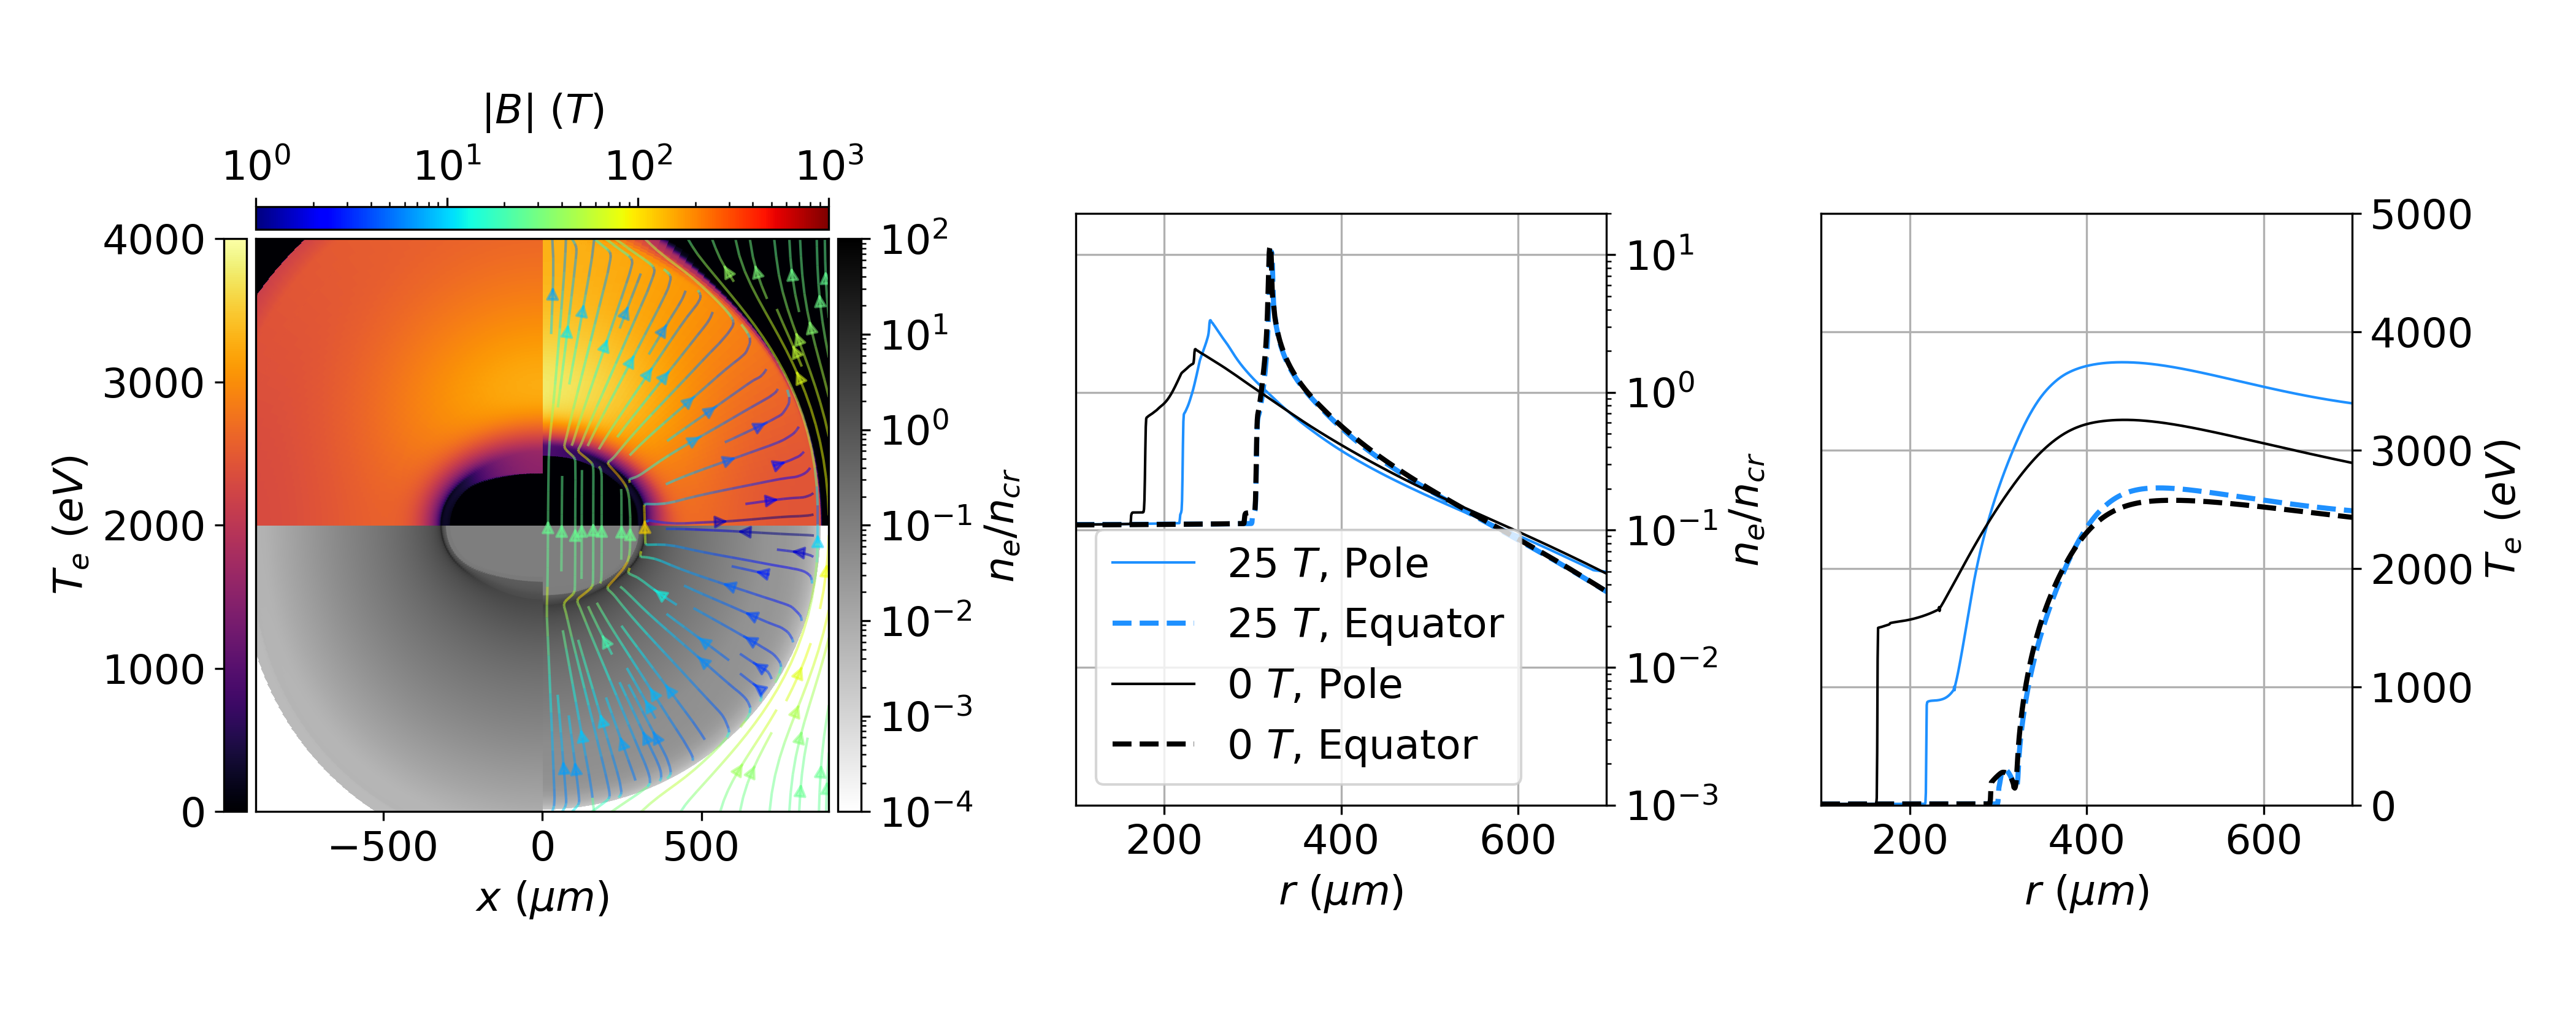
\includegraphics[width=\linewidth]{Results2/Images/ne_te_Bstream_comp_alt050.png}
    \centering
    \caption{Comparison of $n_e$ and $T_e$ profiles from the $B_{z0}=0$ (panel a) left-side) and $25\ \text{T}$ (panel a) right-side), with-\ac{CBET} simulations, both at $t=0.5\ \text{ns}$.
    Panel a) also plots streamlines of $\vec{B}$ for the $B_{z0}=25\ \text{T}$ simulation, coloured by the field magnitude.
    Panels b) and c) plot $n_e$ and $T_e$ lineouts respectively, along both the pole and equator.
    It is evident from these lineouts that magnetisation anisotropically affects hydrodynamic variables, which are used to calculate the \ac{CBET} gain.
    Therefore, it is anticipated that magnetisation could anisotropically affect the \ac{CBET} scattering volume.}%
    \label{fig:Res2_ne_te_Bstream_comp_alt050}
\end{figure}

This section presents results on how the magnetisation of the corona affects both \ac{CBET} scattering and the stagnation shape of the implosion.
As was shown in the previous sections, the laser geometry leads to a significant mode $\ell=2$ in the coronal plasma conditions, which is significantly amplified by anisotropic thermal conduction when magnetised.
This long-wavelength perturbation is slightly reduced by \ac{CBET}, consistent with existing literature on how \ac{CBET} mitigates $\ell=1$ asymmetries~\cite{colaitis_inverse_2021}.
`No-\ac{CBET}' simulations were conducted, for which the coupled energy was kept the same as the equivalent \ac{CBET} simulation, \textit{i.e.} so \ac{CBET} only acted to redistribute the deposited power, rather than reduce its magnitude.
These results showed that the increasingly anisotropic coronal plasma profiles for increasing seed magnetic field strengths did lead to changes in the \ac{CBET} scattering, this was too small an effect to lead to experimentally observable changes in behaviour.

%################################################################################
%################################################################################
\subsection{Analysis and Key Definitions}%
\label{sec:Res2_analysis_definitions}

\begin{figure}[t!]
    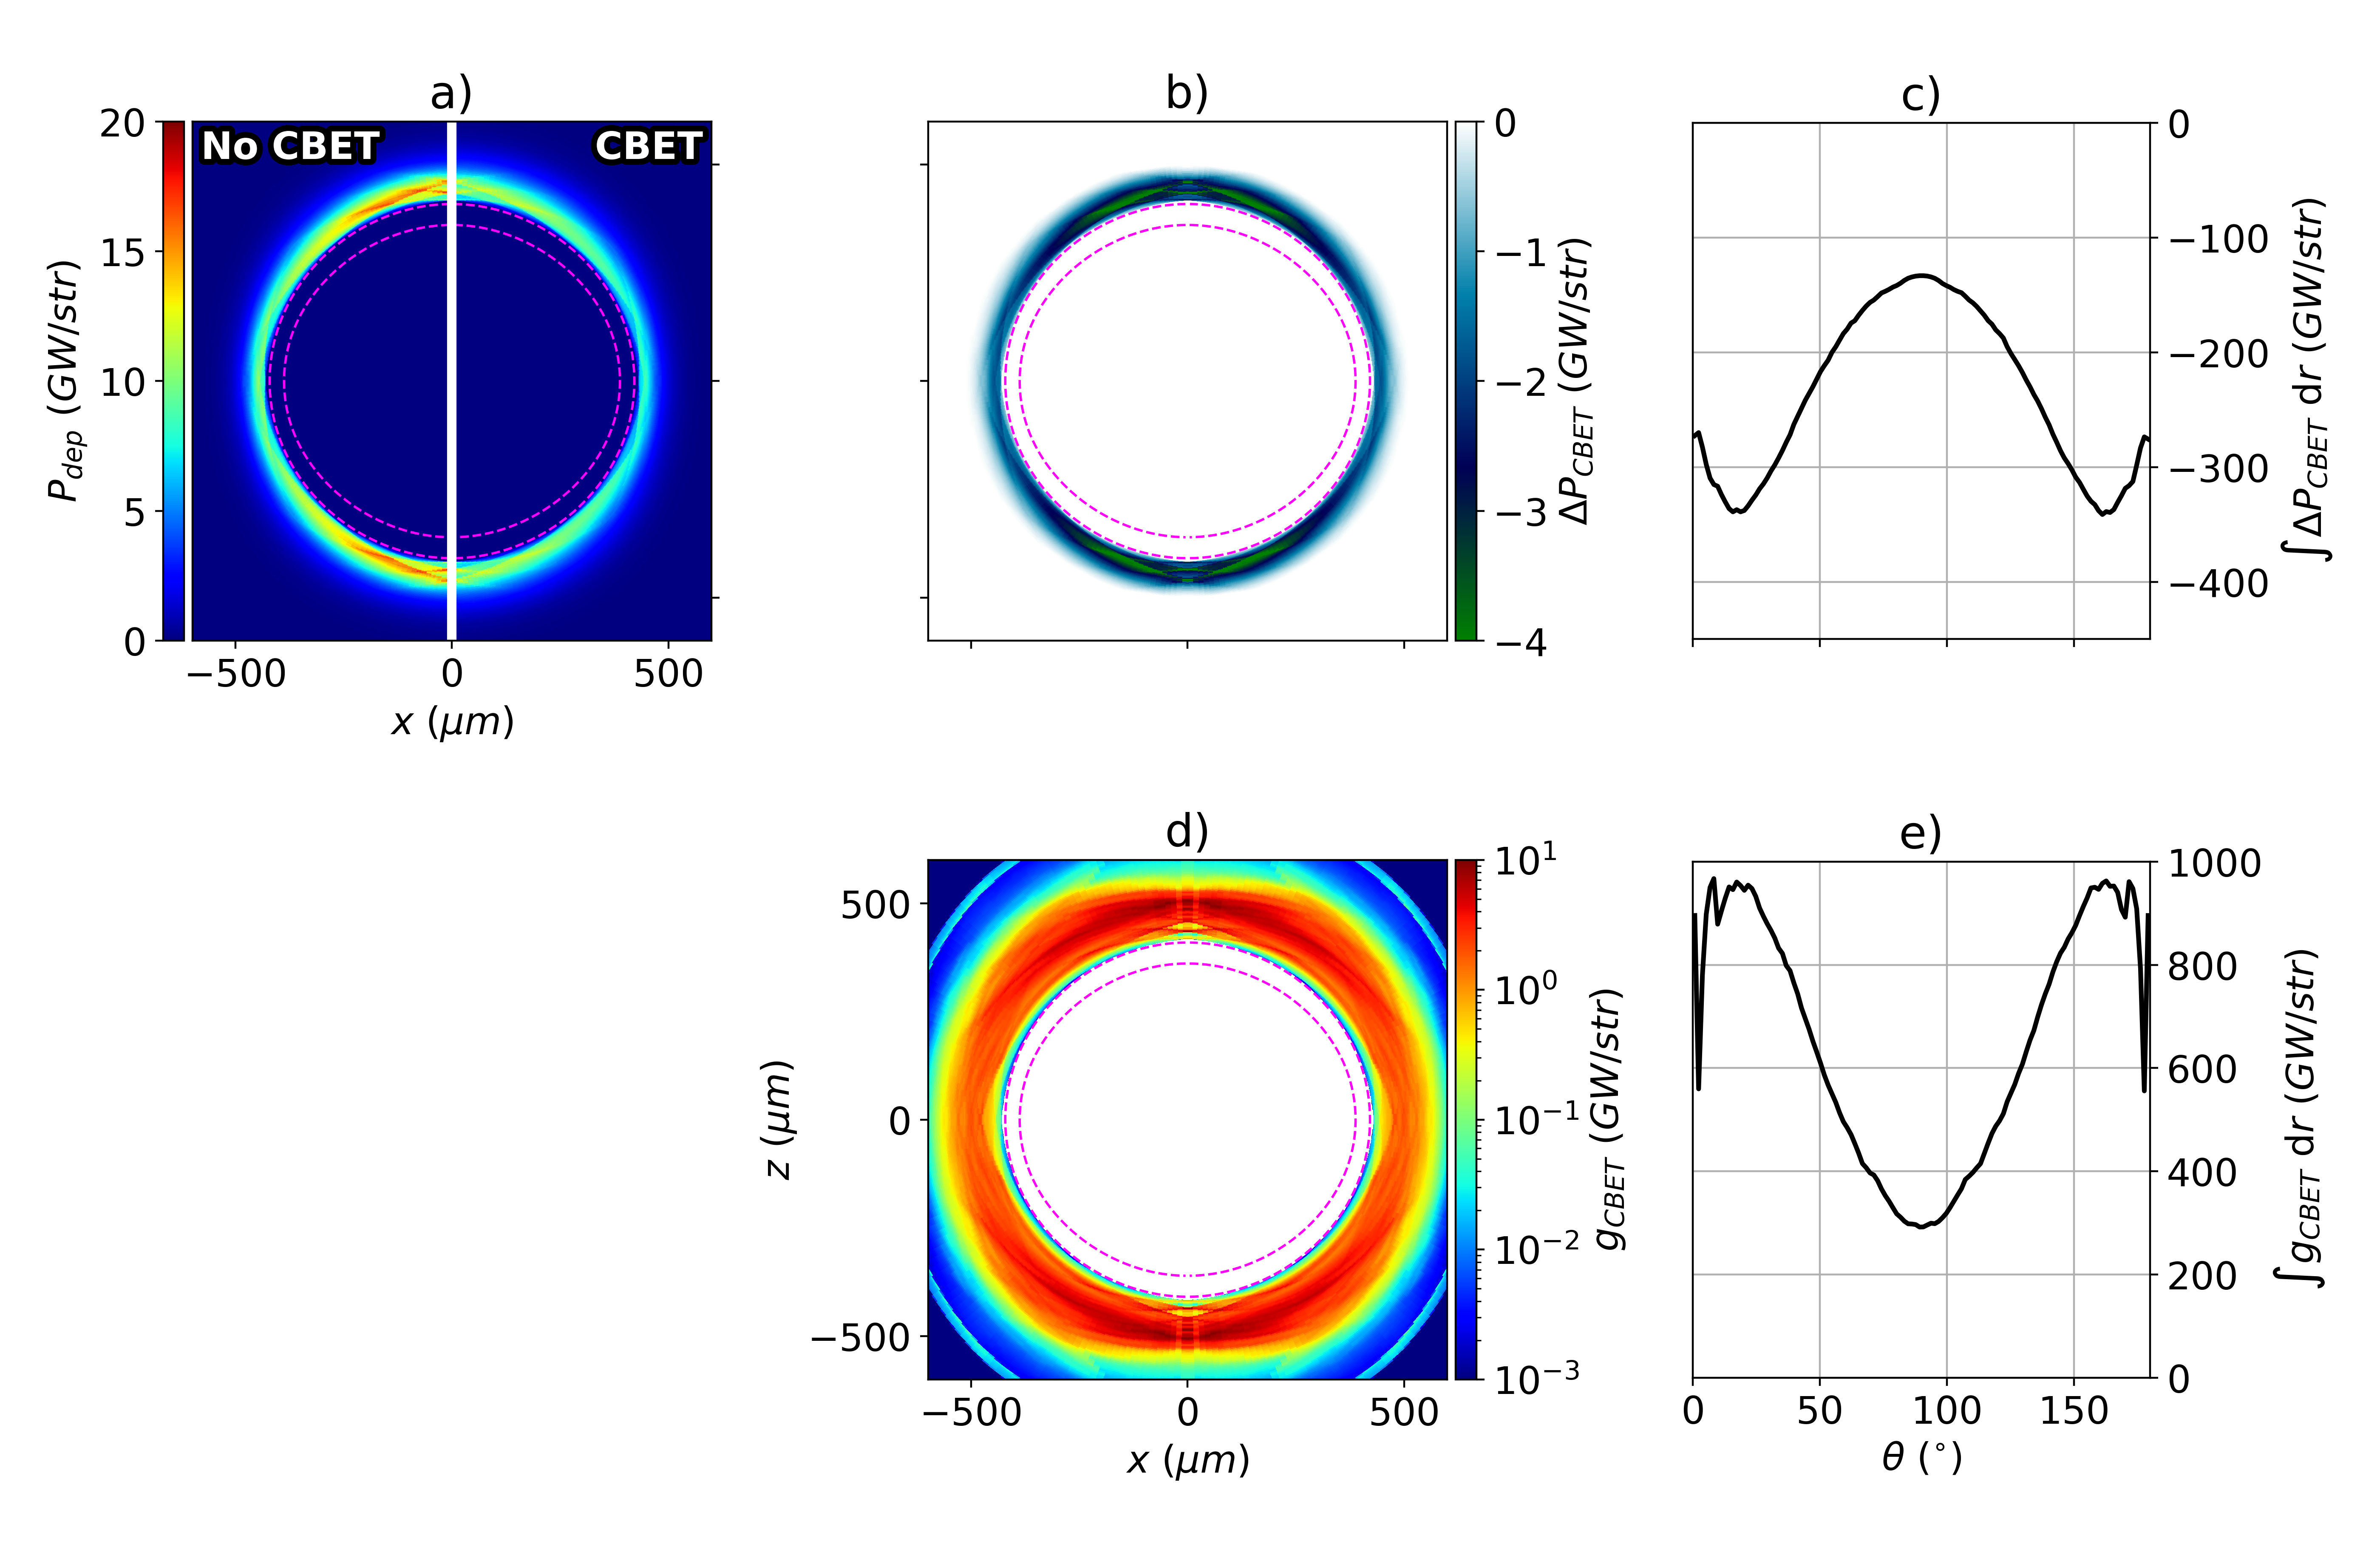
\includegraphics[width=\linewidth]{Results2/Images/magcbet_analysis.png}
    \centering
    \caption{Various \ac{CBET} diagnostics used in the analysis presented in this section.
    All plots are from the $B_{z0}=0\ \text{T}$, with-\ac{CBET} simulation at $t=0.30\ \text{ns}$.
    Panel a) plots the instantaneous deposition with (right-side) and without (left-side) the effect of \ac{CBET}.
    The `\ac{CBET}-deficit', $\Delta P_{\text{CBET}}$, which is the no-\ac{CBET} deposition, subtracted from the with-\ac{CBET} deposition, is plotted in panel b).
    Panel c) plots the radially integrated $\Delta P_{\text{CBET}}$, as a function of polar angle.
    The `\ac{CBET}-scattering', defined in Eq.~\ref{sec:res1_cbet_scattering}, is plotted in panel d), and the radial integral is plotted in panel e).
    At this time, it is evident from panel e) that more \ac{CBET} occurs at the capsule poles, resulting in a \ac{CBET}-reduction of deposition near the poles, seen in panel c).}%
    \label{fig:Res2_magcbet_analysis}
\end{figure}


%################################################################################
%################################################################################
\subsection{Spatial Change of CBET and Deposition from Magnetisation}%
\label{sec:Res2_mag_on_cbet_change}

\begin{figure}[t!]
    \includegraphics[width=\linewidth]{Results2/Images/Scattering_time_phi_diffCBET_CBtr.png}
    \centering
    \caption{The radially integrated \ac{CBET}-deficit and \ac{CBET}-scattering, plotted as a function of angle and time for the $B_{z0}=0$ and $50\ \text{T}$, with-\ac{CBET} simulations.
    Panel b) plots the \ac{CBET}-deficit from the 50 T (top-half) and 0 T (bottom-half) simulations.
    Lineouts in $\theta$ at $t=0.25$ (black), $0.50$ (dark-green) and $0.75\ \text{ns}$ (light-green) are plotted in panel a).
    The same results, but for \ac{CBET}-scattering are plotted in panels d) and c).
    It is evident from these plots that for both simulations, as time progresses and the poles of the capsule fall in faster than the equator, the region where \ac{CBET} mostly occurs, shifts in angle around the capsule.
    Differences are visible in all plots between the $B_{z0}=0$ and $50\ \text{T}$ simulations, indicating that magnetisation affected \ac{CBET} indirectly, via the altered hydrodynamics.}%
    \label{fig:Res2_scattering}
\end{figure}

%################################################################################
%################################################################################
\subsection{Stagnation Profiles}%
\label{sec:Res2_stgnation_profiles}


\begin{figure}[t!]
    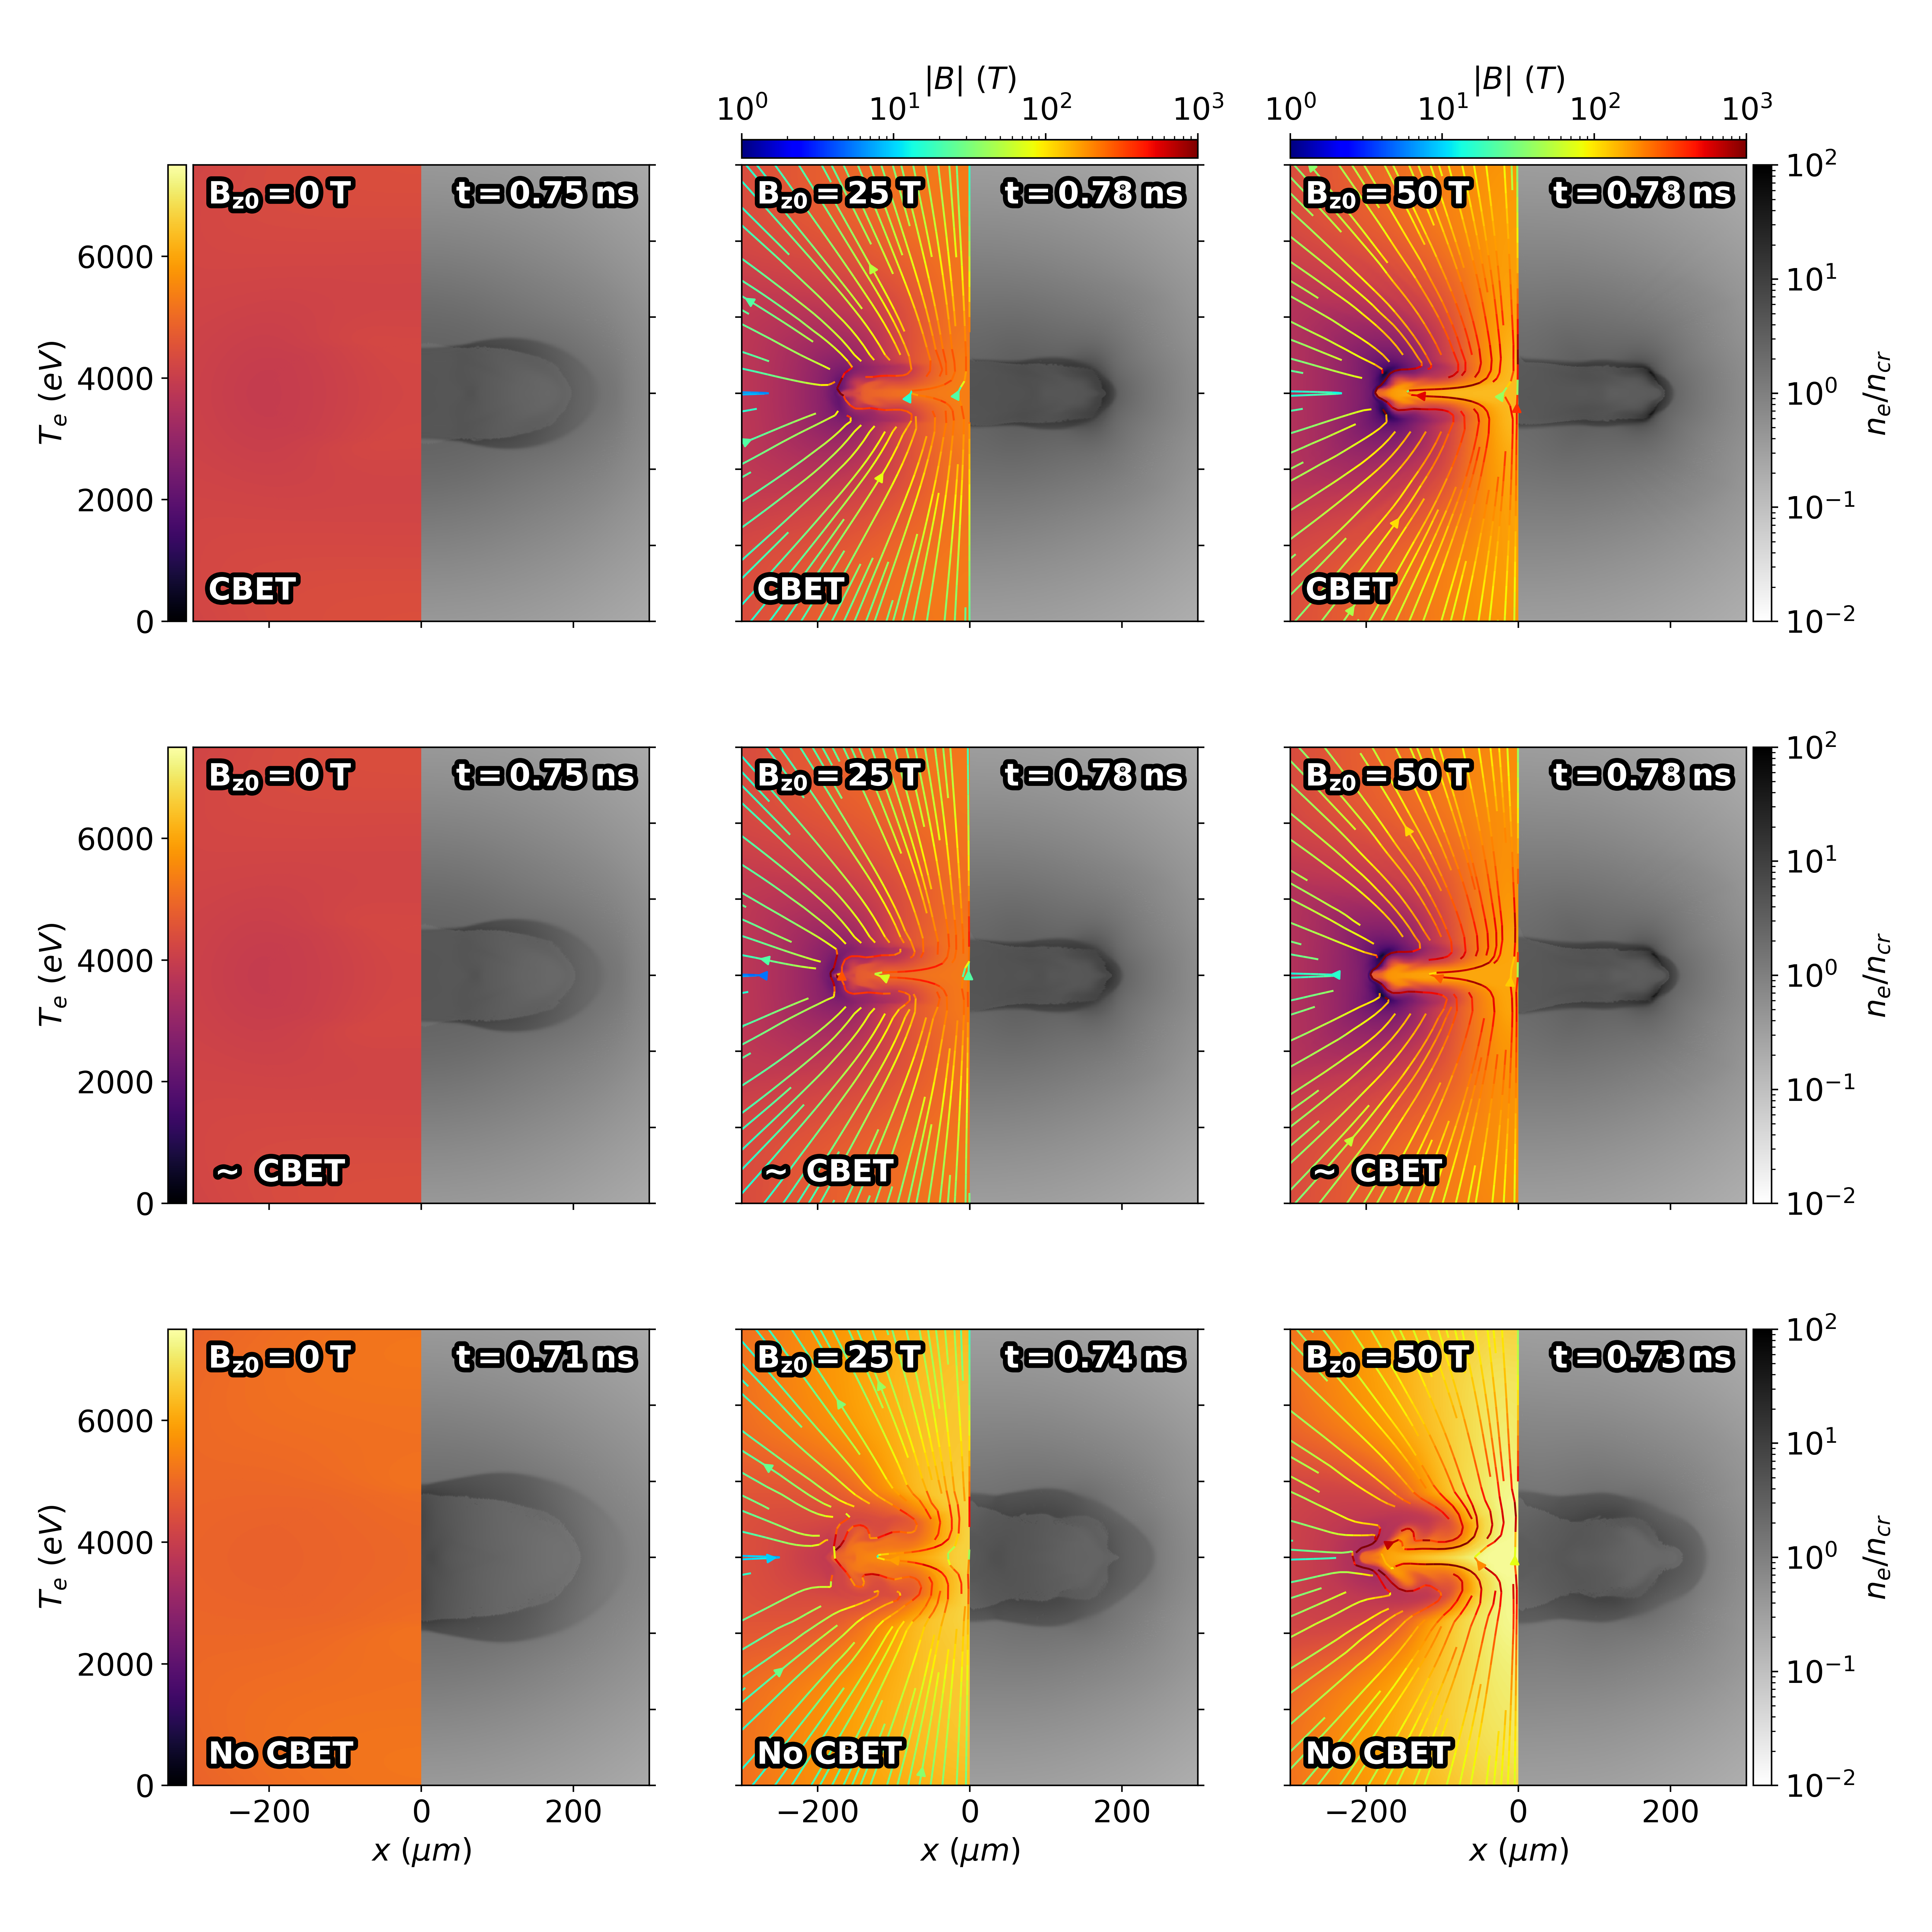
\includegraphics[width=\linewidth]{Results2/Images/allall_stagnation.png}
    \centering
    \caption{$n_e$, $T_e$ and $\vec{B}$ profiles from the time of peak neutron production for different initial magnetisation (columns) and \ac{CBET} effects (rows).
    Panels a), b) and c) are from the full \ac{CBET} simulations, which show that magnetisation increases the oblateness of the stagnation profile.
    Panels d), e) and f) are from the simulations where only the \ac{CBET} effect on the magnitude, but not spatial location, of deposition was included.
    These simulations have identical coupled energy to the top row, and therefore have the same bangtimes.
    Panels g), h) and i) are from the no-\ac{CBET} simulations, which have earlier bangtimes and increased temperatures due to the higher coupled energy.}%
    \label{fig:Res2_allall_stagnation}
\end{figure}

If \ac{CBET} was anisotropically affected by magnetisation, this would result in spatial differences in deposition location, between the full \ac{CBET} (top row) and \ac{CBET}-on-magnitude simulations (middle row), and therefore the bangtime profiles could be different.
Additionally, higher initial magnetisation increases the anisotropy of the coronal plasma and therefore 

\begin{figure}[t!]
    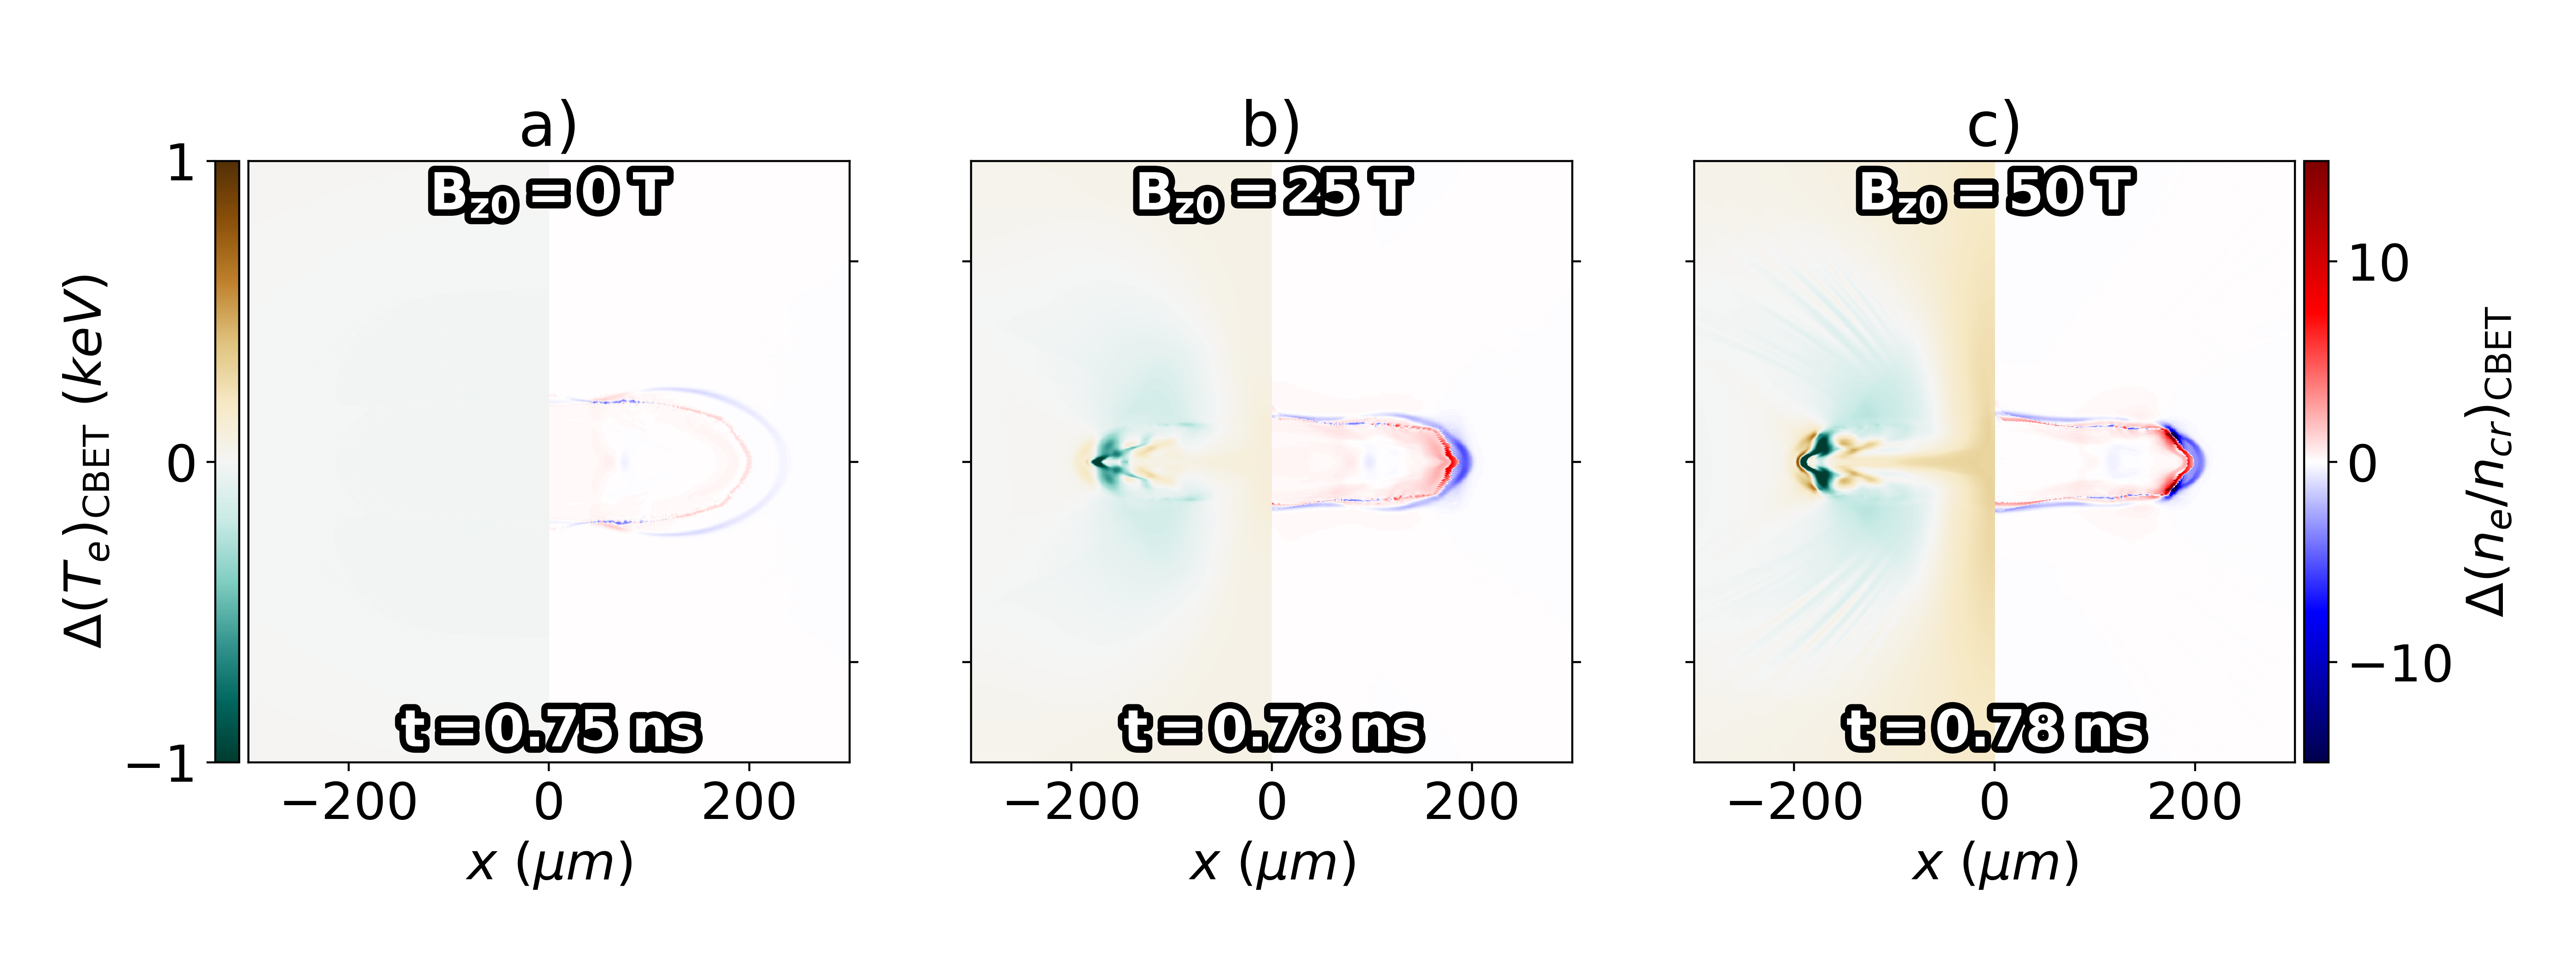
\includegraphics[width=\linewidth]{Results2/Images/CBETshape_stag_diff.png}
    \centering
    \caption{Difference in $n_e$ and $T_e$ bangtime profiles, between the full-\ac{CBET} and \ac{CBET}-magnitude a) $B_{z0}=0$, b) $B_{z0}=25$ and c) $B_{z0}=50\ \text{T}$ simulations.
    The difference in variable $v$, $\Delta v$ is the $v_{full-CB}-v_{mag_CB}$, so higher colour scale values represent regions with increased $v$ for the full \ac{CBET} calculation.
    These results primarily show that \ac{CBET} slightly reduces the bangtime equatorial radius, and thus reduces the oblateness, compared to simulations where the spatial redistribution of power due to \ac{CBET} is neglected.}%
    \label{fig:Res2_CBETshape_diff}
\end{figure}

\begin{figure}[t!]
    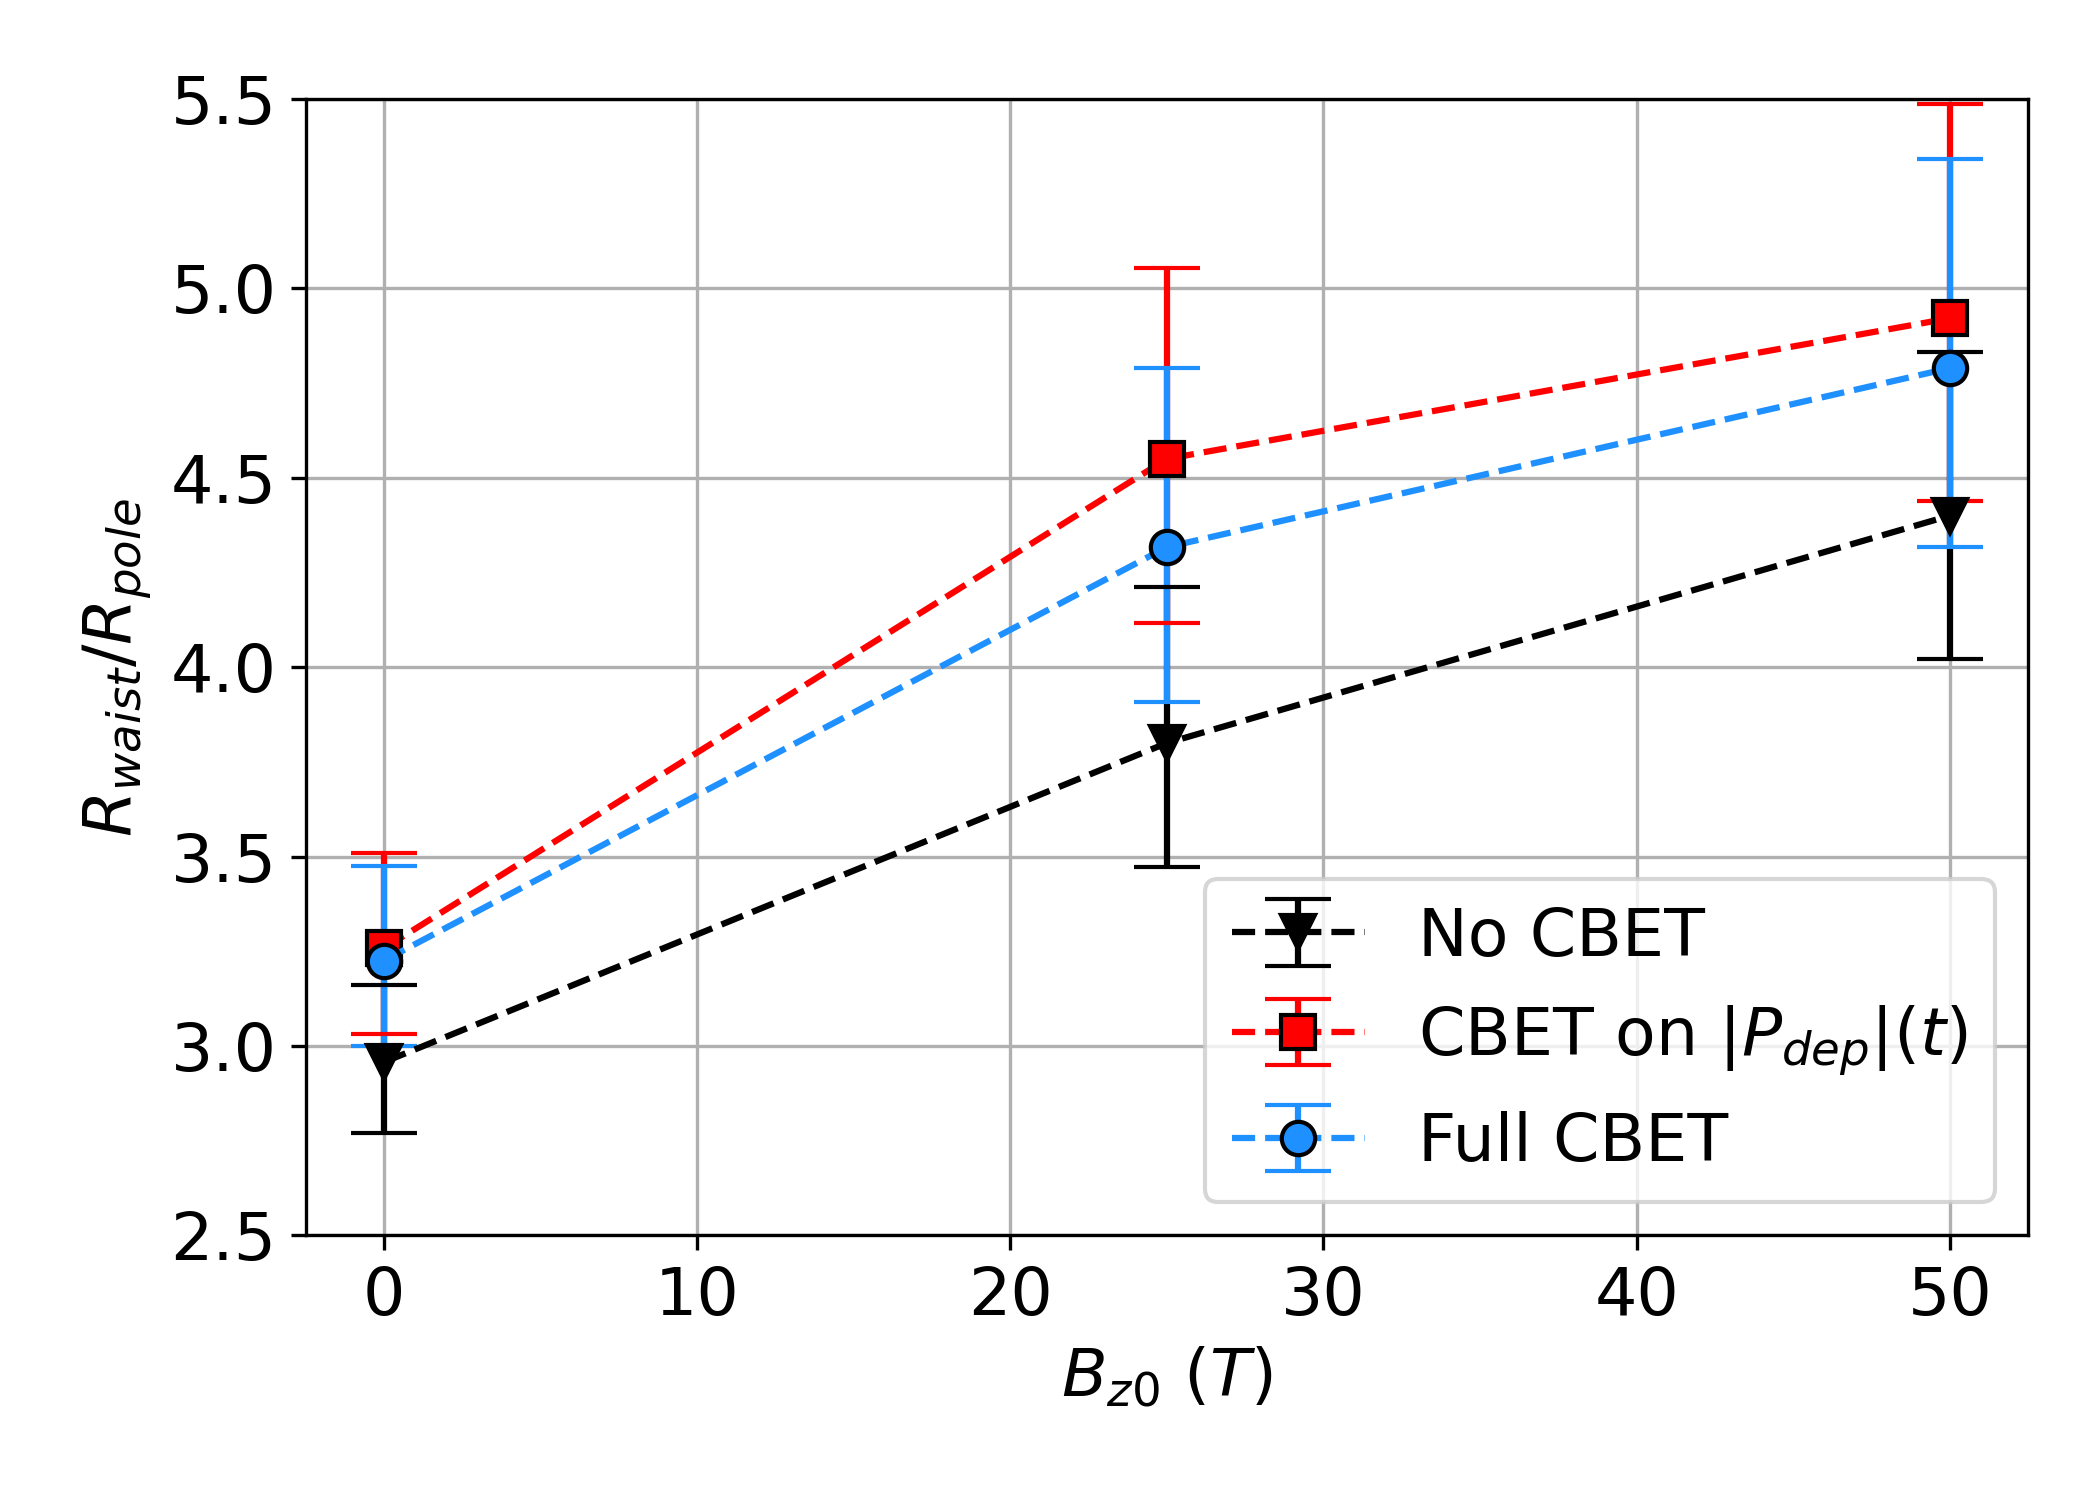
\includegraphics[width=0.6\linewidth]{Results2/Images/R2R0_errors.png}
    \centering
    \caption{The oblateness of bangtime density profiles for different magnetisation and \ac{CBET} effects.
    All values and errors were obtained by fitting an ellipse (with axes orientated along $\hat{\vec{x}}$ and $\hat{\vec{z}}$), to the radius of maximum density.
    No-\ac{CBET} simulations are consistently more round, because the initial shock is stronger and therefore travels ahead of the pusher material more quickly than the \ac{CBET} equivalent.
    Thus, after rebounding off the axis, it meets the infalling mass and produces thermonuclear conditions at a larger radius.
    As was seen in Fig.~\ref{fig:Res2_CBETshape_diff}, throughout the entire implosion, when including the effect of \ac{CBET} on spatial location of deposition, it acts to slightly move energy from the pole to the waist and thus marginally reduces oblateness of the implosion.}%
    \label{fig:Res2_R2R0_errors}
\end{figure}



%###############################################################################################################################
%###############################################################################################################################
%###############################################################################################################################
\section{Conclusions}%
\label{sec:Res2_conclusions}



%################################################################################
%################################################################################
\subsection{Summary of Work}%
\label{sec:Res2_summary}



%################################################################################
%################################################################################
\subsection{Future Work}%
\label{sec:Res2_future}

